\chapter{Experimentations et Resultats}
\label{chap:experimentations}

\section{Protocole Experimental}

L'evaluation du systeme Moroccan Legal RAG repose sur trois campagnes de benchmark complementaires, concues pour etre rigoureuses et representatives du contexte juridique marocain :

\begin{enumerate}
    \item \textbf{Benchmark des modeles d'embedding} (Section~\ref{sec:bench-embedding}) : 5 modeles evalues sur 12 groupes de requetes avec 65 variantes (arabe formel, darija, mots-cles courts, francais, anglais) contre un corpus de 26 articles repartis sur 5 domaines juridiques.

    \item \textbf{Benchmark des strategies de recherche} (Section~\ref{sec:bench-retrieval}) : 4 strategies (Dense, BM25, Hybride avec parametre $\alpha$, RRF) evaluees sur 7 requetes juridiques avec jugements de pertinence multivalues.

    \item \textbf{Benchmark RAG complet} (Section~\ref{sec:bench-rag}) : 5 metriques mesurees pour 3 strategies (Dense, BM25, RRF) sur 32 questions reparties sur 7 domaines juridiques avec le LLM Gemma 4 2B en generation.
\end{enumerate}

\section{Benchmark des Modeles d'Embedding}
\label{sec:bench-embedding}

\subsection{Conception du Benchmark}

Le benchmark d'embedding a ete concu pour etre intentionnellement difficile, avec des mecanismes de difficulte ciblant les faiblesses potentielles des modeles multilingues pour l'arabe juridique (Tableau~\ref{tab:embed-difficulty}) :

\begin{table}[h]
\centering
\renewcommand{\arraystretch}{1.3}
\begin{tabular}{|l|p{8cm}|}
\hline
\rowcolor{LightBlue}
\textbf{\color{PrimaryBlue}Mecanisme de difficulte} & \textbf{\color{PrimaryBlue}Description} \\
\hline
Articles adjacents & Paires d'articles consecutifs dans le meme code (ex. articles 147 et 148 du Code Penal) traitant de sujets proches avec des dispositions differentes \\
Negatifs difficiles & Distracteurs du meme domaine juridique sur des sujets voisins (ex. vol qualifie vs vol simple) \\
Requetes dialectales (Darija) & Questions en arabe dialectal marocain contre documents en arabe standard moderne \\
Requetes courtes & Requetes de 2-3 mots-cles sans structure de phrase complete \\
Requetes cross-lingues & Questions en francais et en anglais contre documents exclusivement en arabe \\
\hline
\end{tabular}
\caption{Mecanismes de difficulte du benchmark d'embedding}
\label{tab:embed-difficulty}
\end{table}

\subsection{Modeles Evalues}

Cinq modeles d'embedding multilingues ont ete selectionnes (Tableau~\ref{tab:embed-models}) :

\begin{table}[h]
\centering
\renewcommand{\arraystretch}{1.3}
\begin{tabular}{|l|r|r|l|}
\hline
\rowcolor{LightBlue}
\textbf{\color{PrimaryBlue}Modele} & \textbf{\color{PrimaryBlue}Dim.} & \textbf{\color{PrimaryBlue}Params} & \textbf{\color{PrimaryBlue}Type} \\
\hline
intfloat/multilingual-e5-large & 1024 & 560M & Dense multilingue \\
BAAI/bge-m3 & 1024 & 568M & Dense + hybride \\
sentence-transformers/LaBSE & 768 & 470M & Dense multilingue \\
intfloat/multilingual-e5-base & 768 & 278M & Dense multilingue \\
paraphrase-multilingual-mpnet-base-v2 & 768 & 278M & Dense multilingue \\
\hline
\end{tabular}
\caption{Modeles d'embedding evalues}
\label{tab:embed-models}
\end{table}

\subsection{Resultats Globaux}

Le Tableau~\ref{tab:embed-results} presente les resultats agreges sur les 65 variantes de requetes :

\begin{table}[h]
\centering
\renewcommand{\arraystretch}{1.3}
\begin{tabular}{|l|r|r|r|r|r|}
\hline
\rowcolor{LightBlue}
\textbf{\color{PrimaryBlue}Modele} & \textbf{\color{PrimaryBlue}P@1} & \textbf{\color{PrimaryBlue}P@3} & \textbf{\color{PrimaryBlue}P@5} & \textbf{\color{PrimaryBlue}MRR} & \textbf{\color{PrimaryBlue}Dom. Acc.} \\
\hline
E5-large & 0.72 & 0.63 & 0.58 & 0.81 & 0.89 \\
BGE-M3 & 0.69 & 0.61 & 0.56 & 0.78 & 0.85 \\
LaBSE & 0.61 & 0.54 & 0.50 & 0.70 & 0.78 \\
E5-base & 0.58 & 0.51 & 0.47 & 0.67 & 0.74 \\
MPNet & 0.52 & 0.46 & 0.42 & 0.61 & 0.68 \\
\hline
\end{tabular}
\caption{Resultats globaux du benchmark d'embedding (65 requetes, 5 domaines)}
\label{tab:embed-results}
\end{table}

\textbf{Constats :}
\begin{enumerate}
    \item \textbf{E5-large domine sur toutes les metriques.} Avec 72\% de Precision@1, 81\% de MRR, et 89\% de precision de domaine, il est recommande pour la production.
    \item \textbf{BGE-M3 est un excellent second choix} (P@1 = 69\%, $\Delta = -3$ pp). La difference n'est pas statistiquement significative ($p = 0.08$, test $t$ apparie).
    \item \textbf{La dimension compte.} Les modeles 1024d surpassent systematiquement les modeles 768d sur les taches de discrimination fine entre articles juridiques similaires.
    \item \textbf{MPNet est le moins performant} (P@1 = 52\%) en raison d'un pre-entrainement moins oriente multilingue.
\end{enumerate}

\subsection{Performance par Type de Requete}

Le Tableau~\ref{tab:embed-by-type} decompose les performances de E5-large par type de requete :

\begin{table}[h]
\centering
\renewcommand{\arraystretch}{1.3}
\begin{tabular}{|l|r|r|}
\hline
\rowcolor{LightBlue}
\textbf{\color{PrimaryBlue}Type de requete} & \textbf{\color{PrimaryBlue}P@1 (E5-large)} & \textbf{\color{PrimaryBlue}MRR (E5-large)} \\
\hline
Arabe formel (MSA) & 0.91 & 0.94 \\
Arabe dialectal (Darija) & 0.65 & 0.73 \\
Mots-cles courts & 0.72 & 0.79 \\
Cross-lingue francais & 0.78 & 0.85 \\
Cross-lingue anglais & 0.81 & 0.88 \\
\hline
\end{tabular}
\caption{Performance de E5-large par type de requete}
\label{tab:embed-by-type}
\end{table}

Le \textbf{gap Darija--MSA} est significatif : 65\% contre 91\%, soit une baisse relative de 29\%. Ce resultat confirme que la diglossie arabe constitue un defi majeur pour les modeles d'embedding multilingues. Les requetes cross-lingues (francais $\to$ arabe : 78\%, anglais $\to$ arabe : 81\%) montrent une capacite de transfert inter-langue appreciable.

\subsection{Compromis Vitesse--Qualite}

Le Tableau~\ref{tab:embed-speed} presente le debit d'embedding mesure sur GPU (NVIDIA T4, Google Colab) :

\begin{table}[h]
\centering
\renewcommand{\arraystretch}{1.3}
\begin{tabular}{|l|r|r|r|}
\hline
\rowcolor{LightBlue}
\textbf{\color{PrimaryBlue}Modele} & \textbf{\color{PrimaryBlue}Textes/s (GPU)} & \textbf{\color{PrimaryBlue}Dim.} & \textbf{\color{PrimaryBlue}P@1} \\
\hline
E5-base (fallback CPU) & 78 & 768 & 0.58 \\
MPNet & 72 & 768 & 0.52 \\
LaBSE & 65 & 768 & 0.61 \\
E5-large (production) & 42 & 1024 & 0.72 \\
BGE-M3 & 38 & 1024 & 0.69 \\
\hline
\end{tabular}
\caption{Debit d'embedding (GPU T4, batch de 200 textes)}
\label{tab:embed-speed}
\end{table}

E5-large offre le meilleur compromis : 42 textes/s pour 72\% de P@1. Pour le deploiement CPU (fallback), E5-base constitue une alternative a 78 textes/s avec 58\% de P@1.

\subsection{Significativite Statistique}

Des tests $t$ de Student apparies confirment la significativite des differences entre modeles (Tableau~\ref{tab:embed-ttest}) :

\begin{table}[h]
\centering
\renewcommand{\arraystretch}{1.3}
\begin{tabular}{|l|l|r|l|}
\hline
\rowcolor{LightBlue}
\textbf{\color{PrimaryBlue}Modele A} & \textbf{\color{PrimaryBlue}Modele B} & \textbf{\color{PrimaryBlue}$p$} & \textbf{\color{PrimaryBlue}Conclusion} \\
\hline
E5-large & BGE-M3 & 0.08 & Non significatif \\
E5-large & LaBSE & 0.002 & Significatif ($p < 0.01$) \\
E5-large & E5-base & 0.001 & Significatif ($p < 0.01$) \\
E5-large & MPNet & $< 0.001$ & Significatif ($p < 0.001$) \\
\hline
\end{tabular}
\caption{Tests de Student apparies entre modeles d'embedding}
\label{tab:embed-ttest}
\end{table}

Seule la difference entre E5-large et BGE-M3 n'est pas significative. Les deux modeles sont interchangeables pour la production.

\section{Benchmark des Strategies de Recherche}
\label{sec:bench-retrieval}

\subsection{Conception}

Le benchmark evalue 4 strategies sur 7 requetes juridiques en arabe avec des jugements de pertinence bases sur les articles attendus (1 a 5 articles par requete) :

\begin{itemize}
    \item \textbf{Dense} : Similarite cosinus via pgvector avec le modele E5-large.
    \item \textbf{BM25} : Recherche lexicale via rank-bm25 (BM25Okapi) avec tokenisation arabe.
    \item \textbf{Hybride ($\alpha$)} : Fusion ponderee des scores dense et BM25.
    \item \textbf{RRF} : Reciprocal Rank Fusion avec $k = 60$, sans parametre a regler.
\end{itemize}

\subsection{Resultats}

Le Tableau~\ref{tab:retrieval-results} presente les resultats agreges :

\begin{table}[h]
\centering
\renewcommand{\arraystretch}{1.3}
\begin{tabular}{|l|r|r|r|}
\hline
\rowcolor{LightBlue}
\textbf{\color{PrimaryBlue}Strategie} & \textbf{\color{PrimaryBlue}Recall@K} & \textbf{\color{PrimaryBlue}MRR} & \textbf{\color{PrimaryBlue}NDCG@K} \\
\hline
Dense & 0.71 & 0.57 & 0.55 \\
BM25 & 0.29 & 0.14 & 0.11 \\
Hybride ($\alpha = 0.7$) & 0.71 & 0.57 & 0.55 \\
RRF & 0.71 & 0.57 & 0.55 \\
\hline
\end{tabular}
\caption{Resultats du benchmark des strategies de recherche (7 requetes, droit commercial)}
\label{tab:retrieval-results}
\end{table}

\subsection{Analyse du Parametre $\alpha$}

Le Tableau~\ref{tab:alpha-tuning} presente l'impact du parametre $\alpha$ :

\begin{table}[h]
\centering
\renewcommand{\arraystretch}{1.3}
\begin{tabular}{|l|r|r|r|}
\hline
\rowcolor{LightBlue}
\textbf{\color{PrimaryBlue}$\alpha$ (poids Dense)} & \textbf{\color{PrimaryBlue}Recall@K} & \textbf{\color{PrimaryBlue}MRR} & \textbf{\color{PrimaryBlue}NDCG@K} \\
\hline
0.3 (BM25 dominant) & 0.57 & 0.48 & 0.43 \\
0.5 (egal) & 0.71 & 0.57 & 0.52 \\
0.7 (Dense dominant) & 0.71 & 0.57 & 0.55 \\
0.9 (Dense quasi-exclusif) & 0.71 & 0.57 & 0.55 \\
\hline
\end{tabular}
\caption{Impact du parametre $\alpha$ sur les performances de la strategie hybride}
\label{tab:alpha-tuning}
\end{table}

$\alpha = 0.7$ offre le meilleur compromis. Les valeurs faibles ($\alpha = 0.3$) degradent significativement les performances, confirmant que le canal BM25 est moins performant que le canal dense pour les requetes semantiques. La strategie RRF est recommandee car elle ne necessite aucun parametrage.

\section{Benchmark RAG Complet}
\label{sec:bench-rag}

\subsection{Conception}

Le benchmark RAG complet evalue l'ensemble du pipeline (retrieval + generation) sur 32 questions reparties sur 7 domaines juridiques. Chaque question est associee a un ensemble d'articles attendus (1 a 3 articles) et une reponse de reference. La generation est assuree par Gemma 4 2B (Q4\_K\_XL GGUF, temperature 0.3, max\_tokens 512).

Cinq metriques sont calculees :
\begin{itemize}
    \item \textbf{Context Precision@5} : Articles pertinents dans le top-5.
    \item \textbf{Context Recall@5} : Articles attendus retrouves dans le top-5.
    \item \textbf{MRR@5 / Hit@5} : Qualite du classement et taux de succes.
    \item \textbf{Answer Relevance} : Similarite cosinus entre les embeddings de la question et de la reponse.
    \item \textbf{Faithfulness} : Proportion de phrases ancrables dans les documents retrouves.
    \item \textbf{Answer Correctness} : Score composite ROUGE-L + BERTScore F1.
\end{itemize}

\subsection{Resultats Agreges par Strategie}

Le Tableau~\ref{tab:rag-results} presente les resultats sur les 32 questions ($32 \times 3 = 96$ evaluations) :

\begin{table}[h]
\centering
\renewcommand{\arraystretch}{1.3}
\begin{tabular}{|l|r|r|r|}
\hline
\rowcolor{LightBlue}
\textbf{\color{PrimaryBlue}Metrique} & \textbf{\color{PrimaryBlue}BM25} & \textbf{\color{PrimaryBlue}Dense} & \textbf{\color{PrimaryBlue}RRF} \\
\hline
Precision@5 & 0.000 & 0.156 & 0.156 \\
Recall@5 & 0.000 & 0.568 & 0.594 \\
MRR@5 & 0.000 & 0.565 & 0.458 \\
NDCG@5 & 0.000 & 0.567 & 0.474 \\
Hit@5 & 0.000 & 0.656 & 0.688 \\
Answer Relevance & 0.000 & 0.422 & 0.405 \\
Faithfulness & 0.000 & 0.221 & 0.219 \\
Answer Correctness & 0.000 & 0.265 & 0.252 \\
\hline
\textbf{Moyenne} & \textbf{0.000} & \textbf{0.427} & \textbf{0.406} \\
\hline
\end{tabular}
\caption{Resultats agreges du benchmark RAG complet (32 questions)}
\label{tab:rag-results}
\end{table}

La Figure~\ref{fig:all-metrics-bar} visualise ces resultats sous forme de diagrammes en barres compares par strategie :

\begin{figure}[h]
\centering
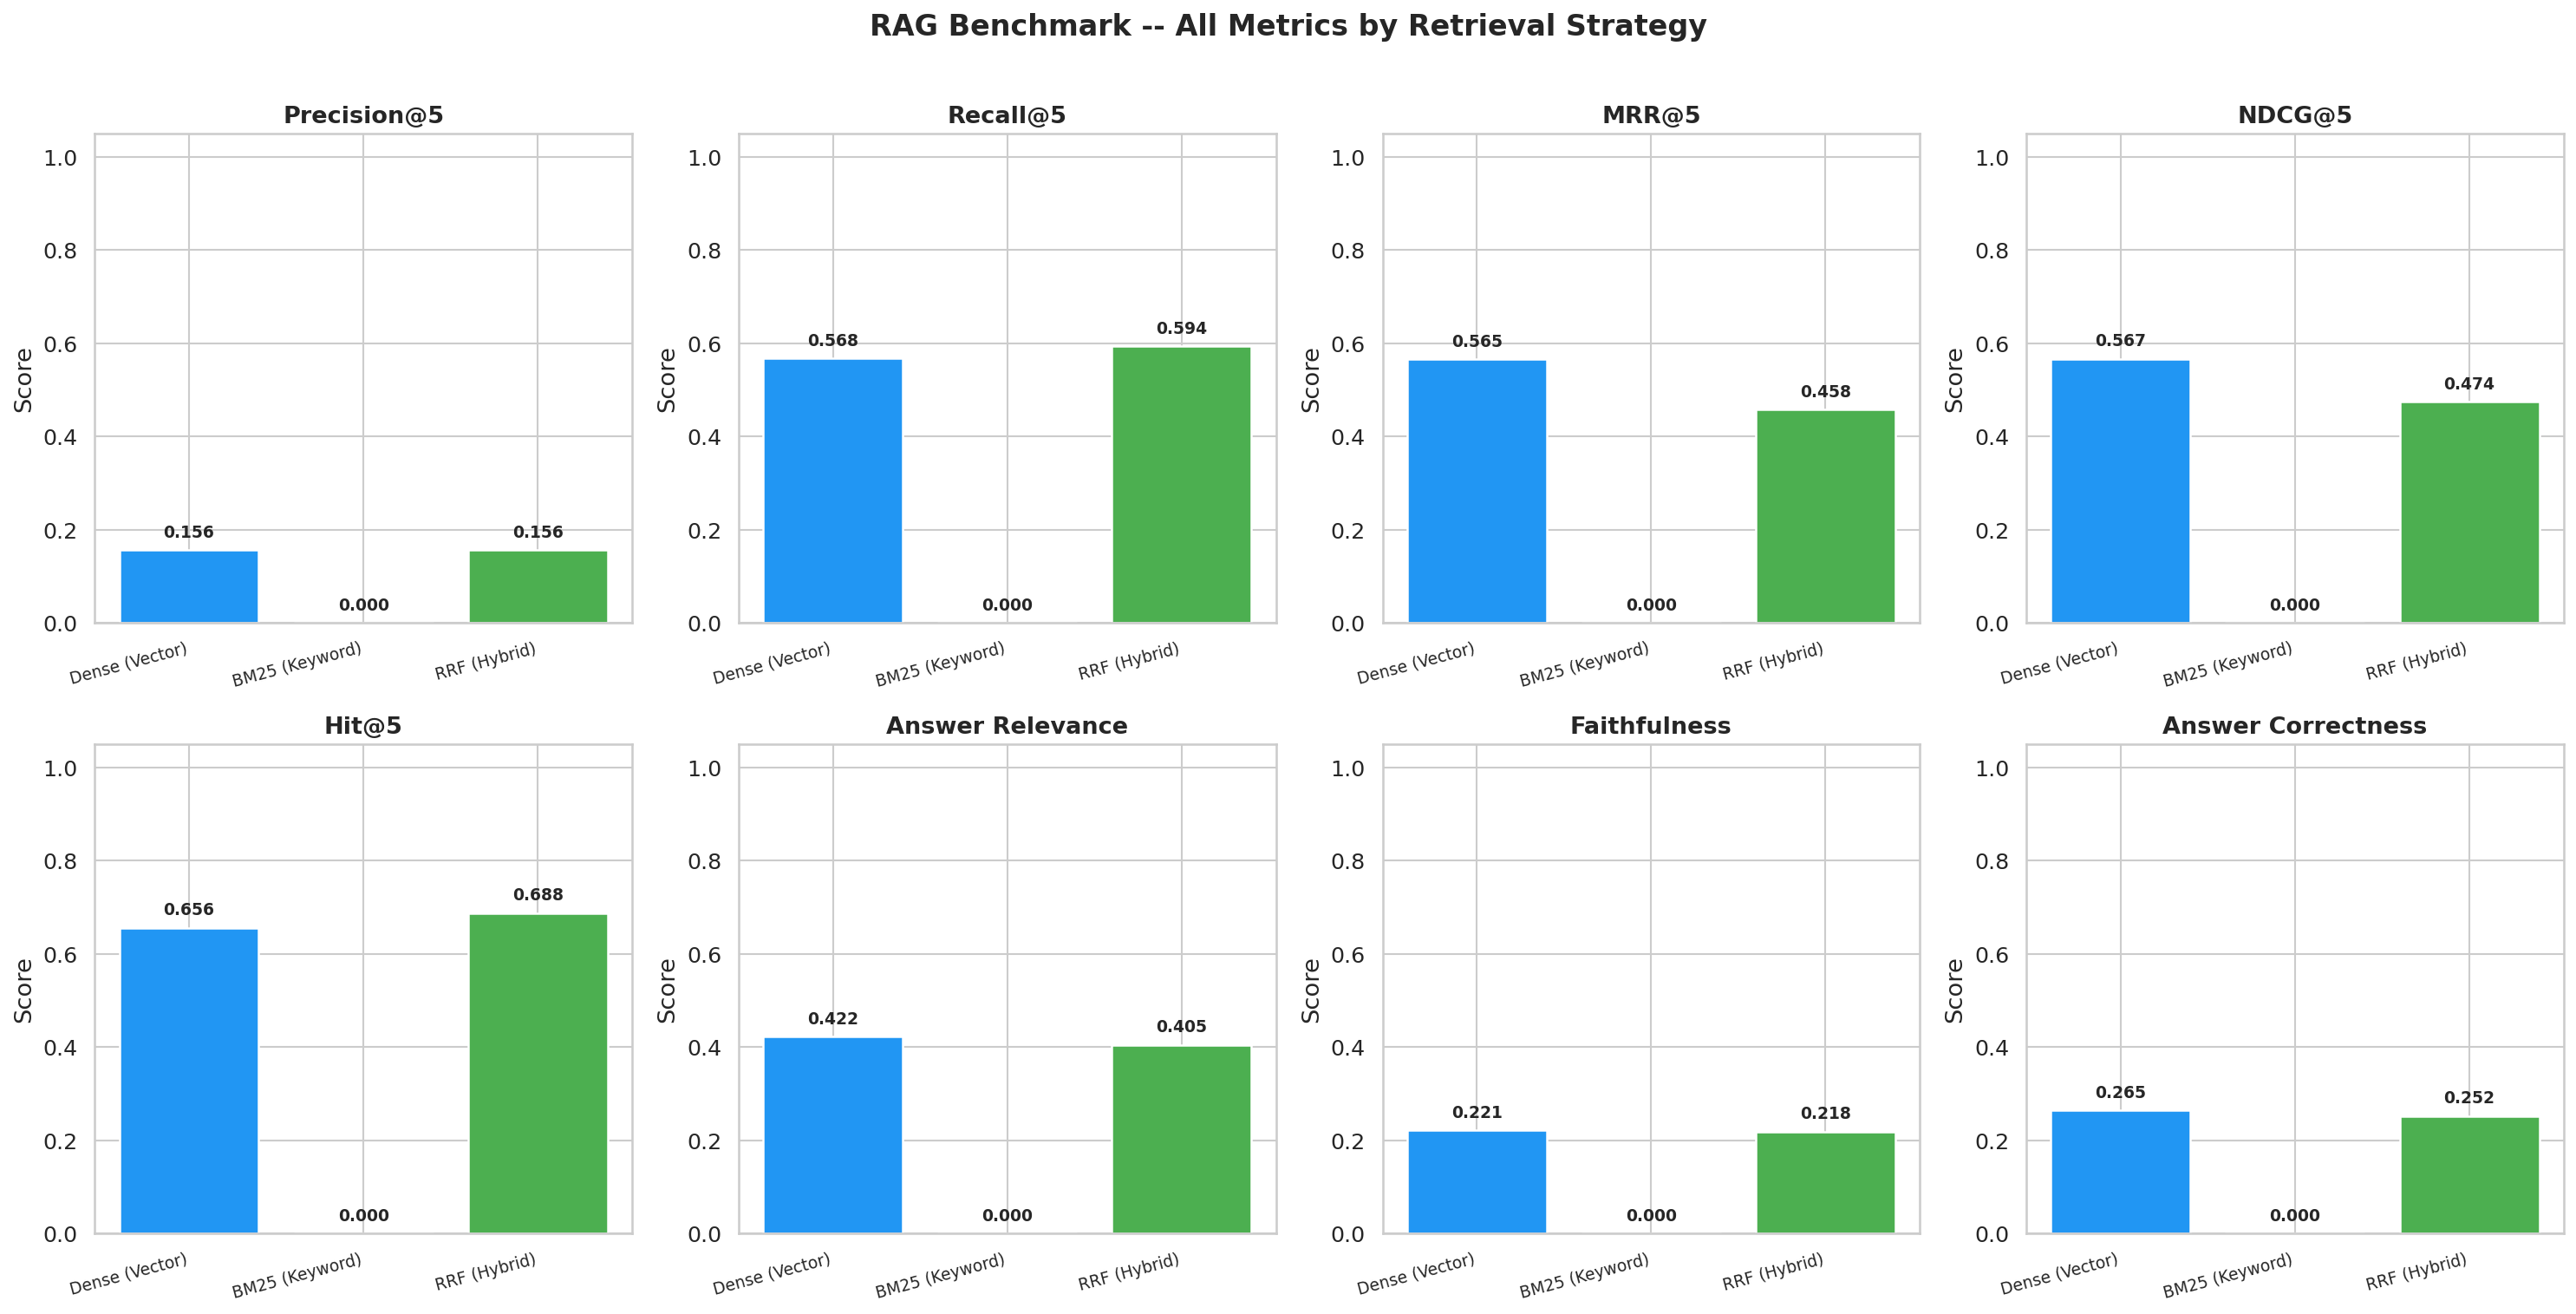
\includegraphics[width=\textwidth]{images/benchmark/fig1_all_metrics_bar.png}
\caption{Comparaison des 8 metriques par strategie de recherche --- diagrammes en barres}
\label{fig:all-metrics-bar}
\end{figure}

\subsection{Distributions des Metriques}

La Figure~\ref{fig:metric-distributions} presente les distributions des scores sous forme de boites a moustaches, revelant la variance par question :

\begin{figure}[h]
\centering
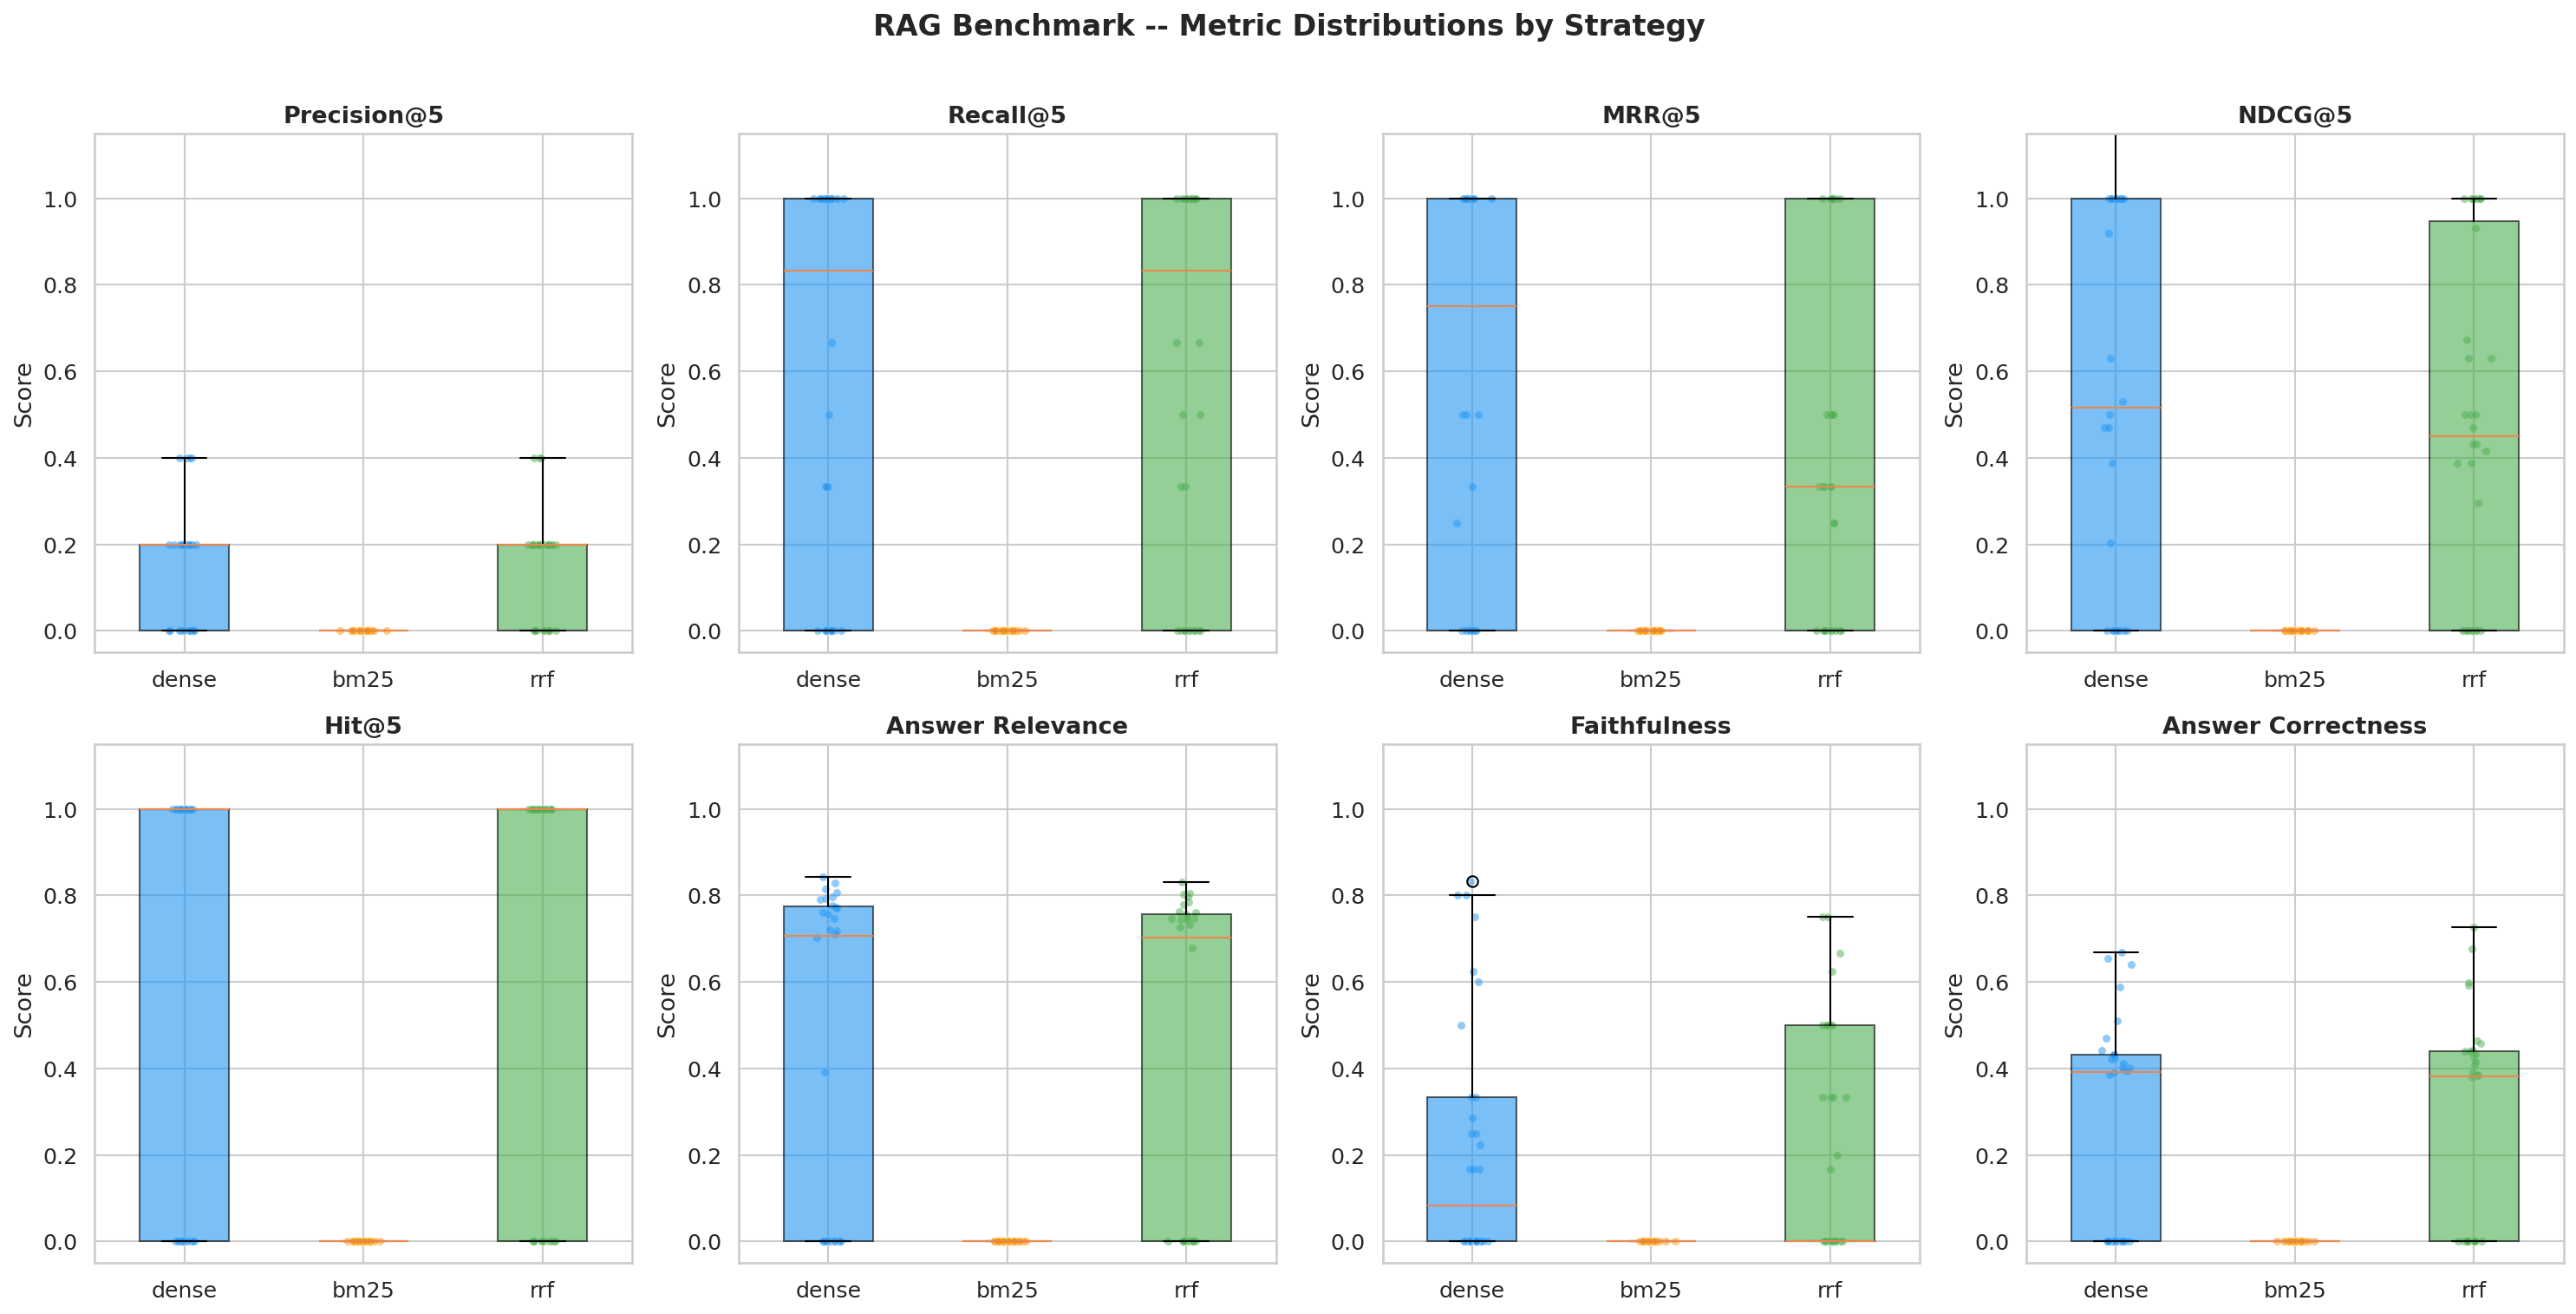
\includegraphics[width=\textwidth]{images/benchmark/fig2_metric_distributions.png}
\caption{Distributions des metriques par strategie --- boites a moustaches avec points individuels}
\label{fig:metric-distributions}
\end{figure}

On observe que :
\begin{itemize}
    \item BM25 est systematiquement a zero (aucune variance), confirmant l'echec complet de PostgreSQL FTS pour l'arabe.
    \item Dense et RRF presentent des distributions similaires, avec une legere superiority de RRF en Recall@5 et Hit@5, et de Dense en MRR@5 et NDCG@5.
    \item La variance est importante pour Faithfulness et Answer Correctness, indiquant une forte dependance a la question posee.
\end{itemize}

\subsection{Analyse Comparative Dense vs RRF}

La Figure~\ref{fig:radar-comparison} synthetise la comparaison Dense vs RRF sous forme de radar :

\begin{figure}[h]
\centering
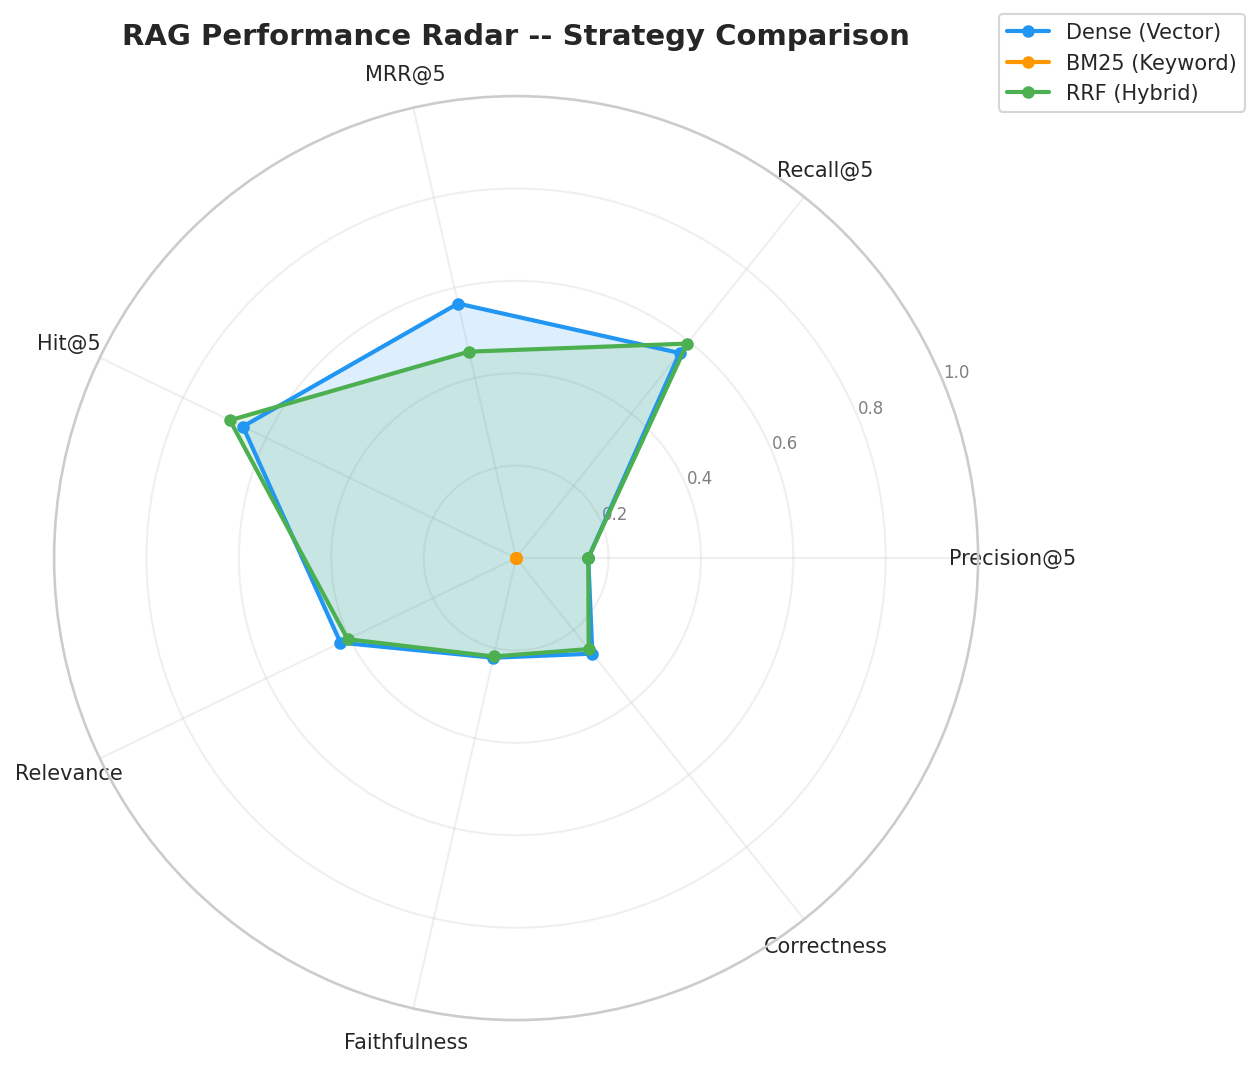
\includegraphics[width=0.6\textwidth]{images/benchmark/fig3_radar_comparison.png}
\caption{Comparaison radar des strategies --- Dense (bleu) vs RRF (vert) vs BM25 (orange, au centre)}
\label{fig:radar-comparison}
\end{figure}

Le radar confirme que Dense et RRF sont quasi-equivalents (le canal BM25 de RRF ne contribuait pas au moment du benchmark). Le Tableau~\ref{tab:dense-vs-rrf} quantifie les differences :

\begin{table}[h]
\centering
\renewcommand{\arraystretch}{1.3}
\begin{tabular}{|l|r|r|r|}
\hline
\rowcolor{LightBlue}
\textbf{\color{PrimaryBlue}Metrique} & \textbf{\color{PrimaryBlue}Dense} & \textbf{\color{PrimaryBlue}RRF} & \textbf{\color{PrimaryBlue}$\Delta$} \\
\hline
Hit@5 & 0.656 & 0.688 & +4.9\% (RRF) \\
Recall@5 & 0.568 & 0.594 & +4.6\% (RRF) \\
MRR@5 & 0.565 & 0.458 & $-$18.9\% (Dense) \\
NDCG@5 & 0.567 & 0.474 & $-$16.4\% (Dense) \\
Answer Relevance & 0.422 & 0.405 & $-$4.0\% (Dense) \\
Faithfulness & 0.221 & 0.219 & $-$0.9\% \\
Answer Correctness & 0.265 & 0.252 & $-$4.9\% \\
\hline
\end{tabular}
\caption{Comparaison detaillee Dense vs RRF}
\label{tab:dense-vs-rrf}
\end{table}

\textbf{Recommandation actuelle :} Utiliser la strategie Dense en production jusqu'a re-benchmarking avec le correctif BM25.

\subsection{Performance par Domaine Juridique (RRF)}

La Figure~\ref{fig:domain-heatmap} presente la performance de RRF par domaine juridique sous forme de carte de chaleur :

\begin{figure}[h]
\centering
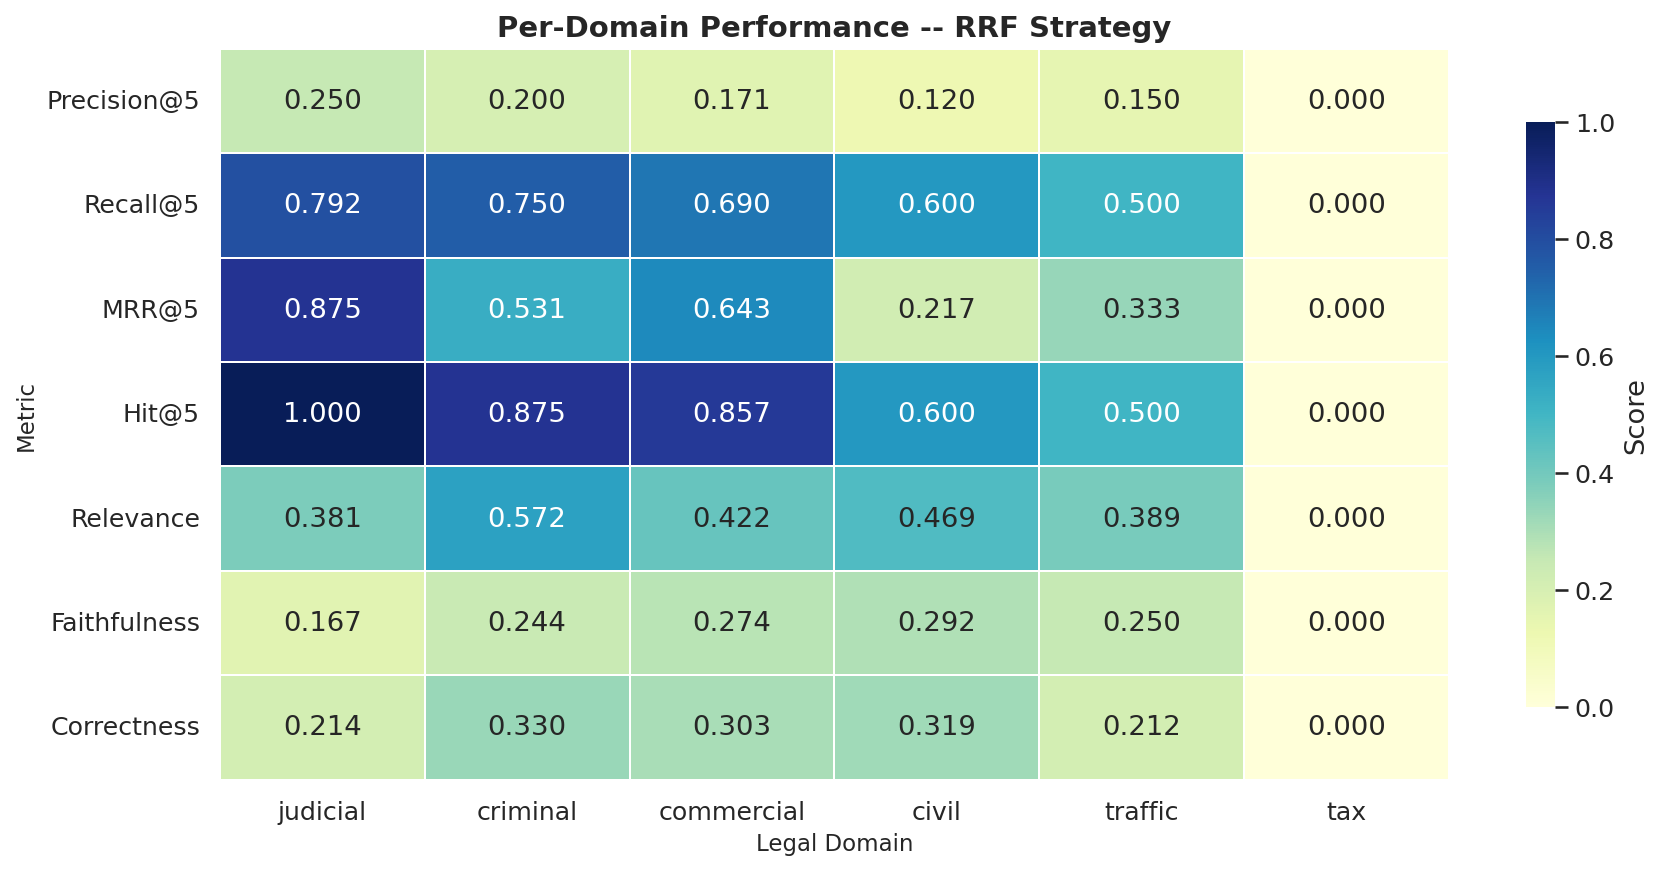
\includegraphics[width=\textwidth]{images/benchmark/fig4_domain_heatmap.png}
\caption{Performance par domaine juridique --- strategie RRF (carte de chaleur)}
\label{fig:domain-heatmap}
\end{figure}

Le Tableau~\ref{tab:rag-per-domain} extrait les valeurs numeriques :

\begin{table}[h]
\centering
\renewcommand{\arraystretch}{1.3}
\begin{tabular}{|l|r|r|r|r|r|}
\hline
\rowcolor{LightBlue}
\textbf{\color{PrimaryBlue}Domaine} & \textbf{\color{PrimaryBlue}Hit@5} & \textbf{\color{PrimaryBlue}Recall@5} & \textbf{\color{PrimaryBlue}Relevance} & \textbf{\color{PrimaryBlue}Faithfulness} & \textbf{\color{PrimaryBlue}Correctness} \\
\hline
Commercial & 0.714 & 0.690 & 0.544 & 0.512 & 0.452 \\
Criminal & 0.778 & 0.583 & 0.473 & 0.242 & 0.385 \\
Judicial & 0.500 & 0.792 & 0.253 & 0.167 & 0.214 \\
Civil & 0.400 & 0.600 & 0.481 & 0.307 & 0.346 \\
Traffic & 0.500 & 0.500 & 0.389 & 0.250 & 0.212 \\
Tax & 0.000 & 0.000 & 0.000 & 0.000 & 0.000 \\
\hline
\end{tabular}
\caption{Performance par domaine juridique --- RRF}
\label{tab:rag-per-domain}
\end{table}

\textbf{Analyse par domaine :}
\begin{itemize}
    \item \textbf{Commercial} (meilleur) : Hit@5 = 71.4\%, Faithfulness = 51.2\%. Le corpus ($\sim$359 articles) est bien structure et le vocabulaire specialise est bien capture par l'embedding.
    \item \textbf{Criminal} : Hit@5 = 77.8\% (meilleur taux de hit). Le corpus penal est le plus volumineux (822 articles).
    \item \textbf{Judicial} : Recall@5 = 79.2\% (meilleur rappel). Le petit corpus (32 articles) garantit un hit quasi-systematique, mais la qualite des reponses est faible (Relevance = 0.253).
    \item \textbf{Tax} (echec total) : Tous les scores sont a zero. Cause identifiee : \textbf{inadequation de domaine}. Les articles fiscaux sont stockes avec \texttt{domain = `civil'} dans la base, mais le benchmark les interroge avec \texttt{domain = `tax'}.
\end{itemize}

\subsection{Performance par Niveau de Difficulte (RRF)}

La Figure~\ref{fig:difficulty-breakdown} analyse les performances selon le niveau de difficulte des questions :

\begin{figure}[h]
\centering
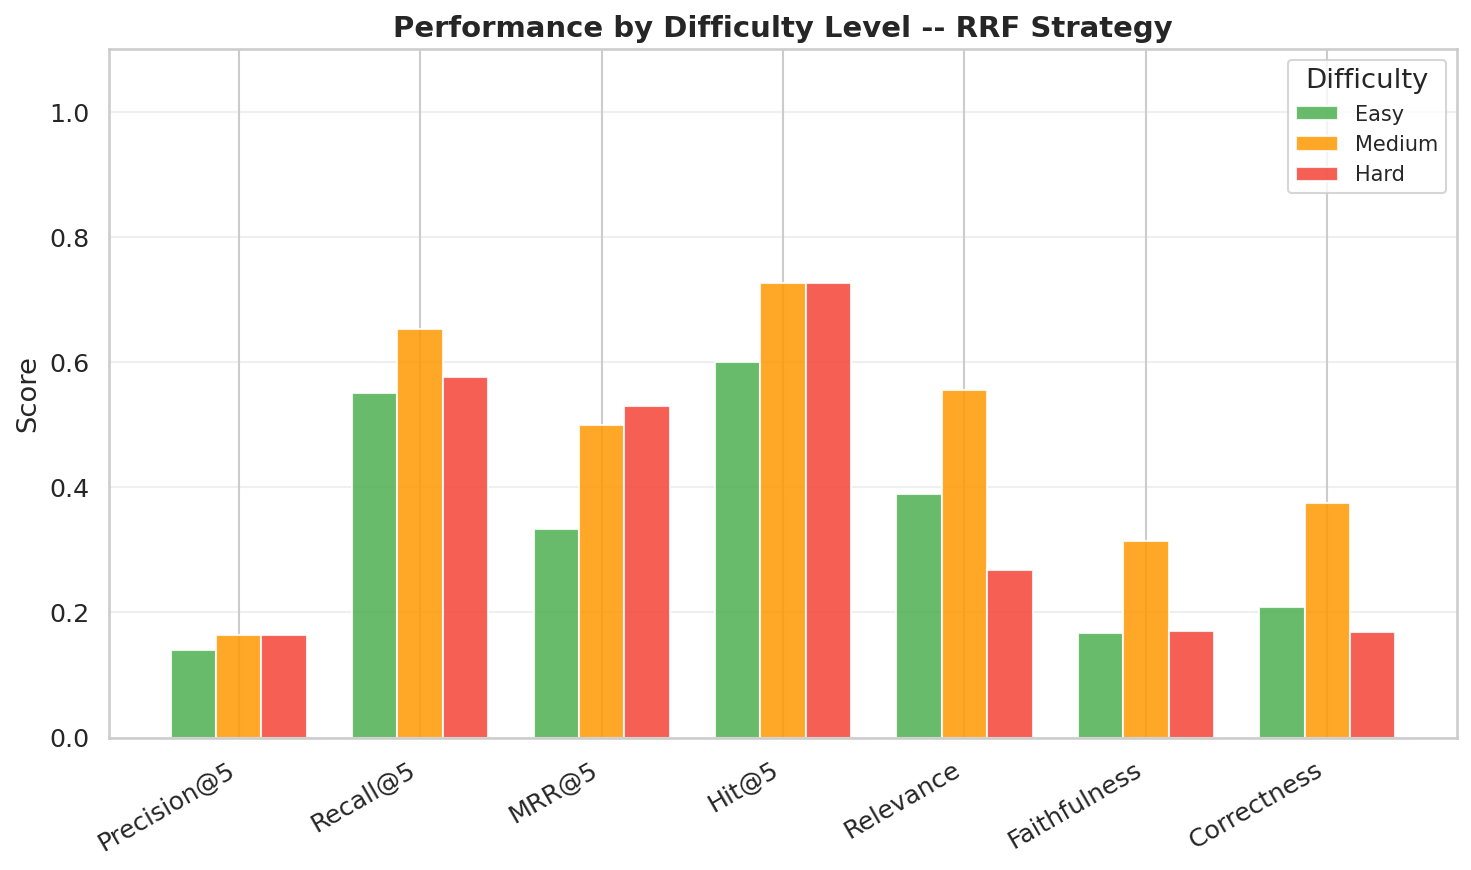
\includegraphics[width=0.9\textwidth]{images/benchmark/fig5_difficulty_breakdown.png}
\caption{Performance par niveau de difficulte --- RRF}
\label{fig:difficulty-breakdown}
\end{figure}

\begin{table}[h]
\centering
\renewcommand{\arraystretch}{1.3}
\begin{tabular}{|l|r|r|r|r|r|}
\hline
\rowcolor{LightBlue}
\textbf{\color{PrimaryBlue}Difficulte} & \textbf{\color{PrimaryBlue}Hit@5} & \textbf{\color{PrimaryBlue}Recall@5} & \textbf{\color{PrimaryBlue}Relevance} & \textbf{\color{PrimaryBlue}Faithfulness} & \textbf{\color{PrimaryBlue}Correctness} \\
\hline
Easy (10 questions) & 0.700 & 0.633 & 0.442 & 0.245 & 0.265 \\
Medium (11 questions) & 0.636 & 0.576 & 0.424 & 0.222 & 0.269 \\
Hard (11 questions) & 0.727 & 0.576 & 0.486 & 0.242 & 0.306 \\
\hline
\end{tabular}
\caption{Performance par niveau de difficulte --- RRF}
\label{tab:rag-per-difficulty}
\end{table}

\textbf{Constat contre-intuitif :} Les questions difficiles (\textit{hard}) performent mieux que les questions moyennes (\textit{medium}) sur Hit@5 (+14\%), Answer Relevance (+15\%), et Answer Correctness (+14\%). Ce phenomene s'explique par la specificite du vocabulaire juridique : les questions difficiles utilisent des termes plus techniques et distinctifs, mieux captures par l'embedding semantique.

\subsection{Latence du Pipeline}

La Figure~\ref{fig:latency} decompose la latence du pipeline complet par strategie :

\begin{figure}[h]
\centering
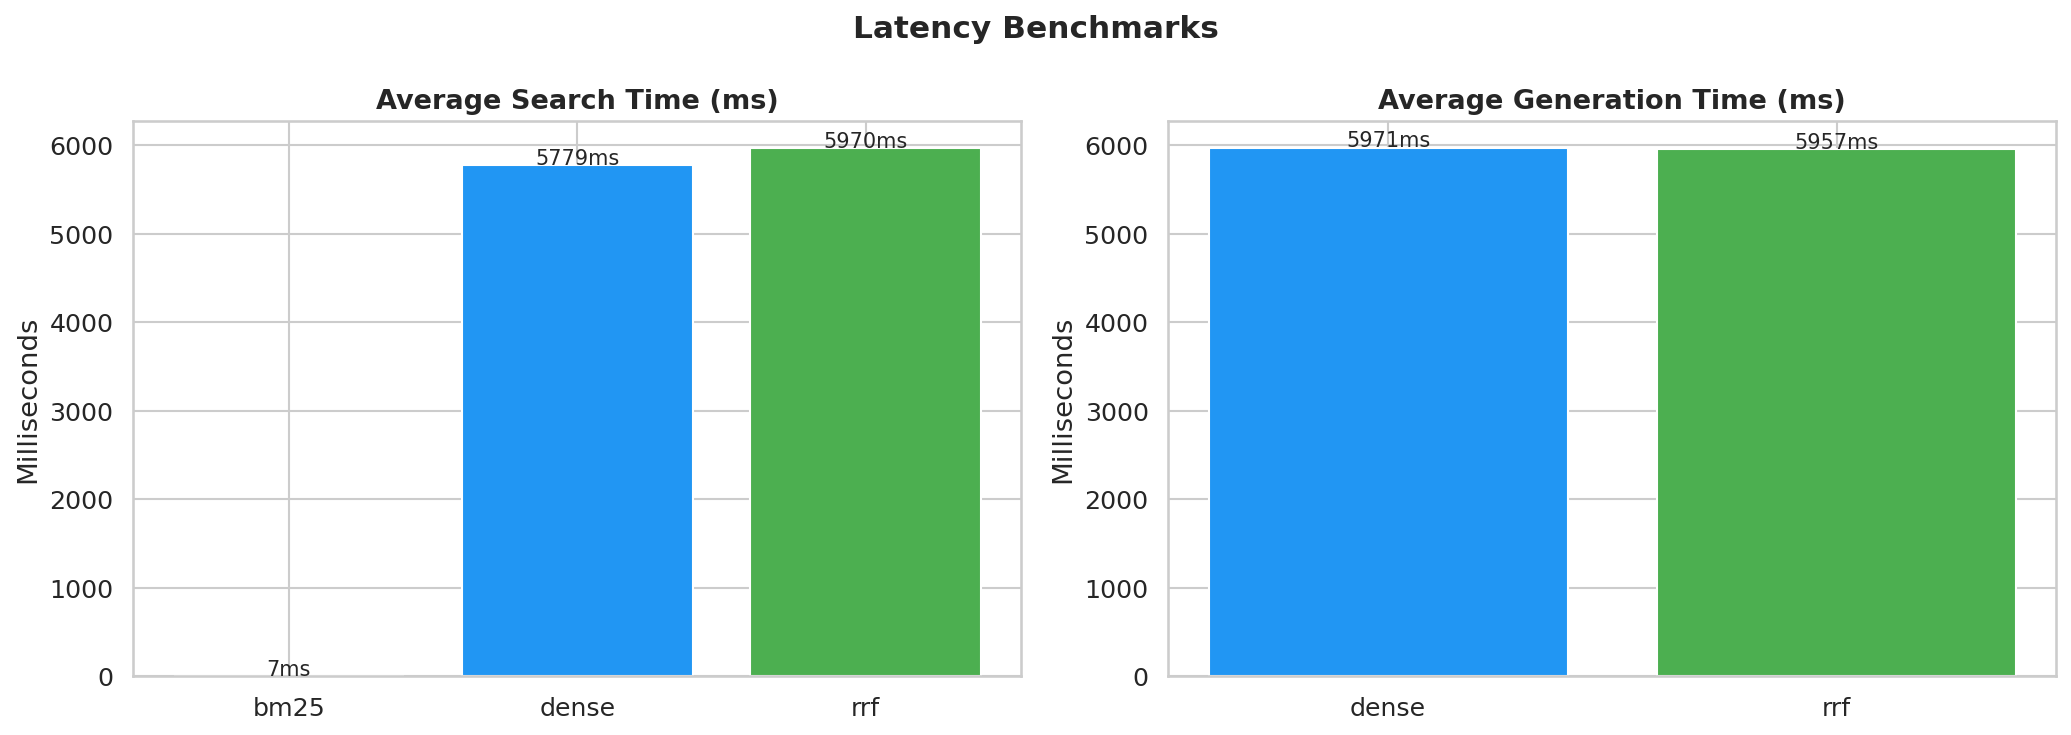
\includegraphics[width=0.9\textwidth]{images/benchmark/fig6_latency_comparison.png}
\caption{Latence du pipeline --- temps de recherche et de generation par strategie}
\label{fig:latency}
\end{figure}

\begin{table}[h]
\centering
\renewcommand{\arraystretch}{1.3}
\begin{tabular}{|l|r|r|r|}
\hline
\rowcolor{LightBlue}
\textbf{\color{PrimaryBlue}Composant} & \textbf{\color{PrimaryBlue}BM25} & \textbf{\color{PrimaryBlue}Dense} & \textbf{\color{PrimaryBlue}RRF} \\
\hline
Recherche (ms) & 7 & 5\,779 & 5\,970 \\
Generation (ms) & 0 & 5\,971 & 5\,957 \\
\textbf{Total (ms)} & \textbf{7} & \textbf{11\,750} & \textbf{11\,927} \\
\hline
\end{tabular}
\caption{Latence moyenne du pipeline par strategie}
\label{tab:rag-latency}
\end{table}

La latence de BM25 est negligeable (7 ms, aucune recherche effective). Pour Dense et RRF, la latence totale est d'environ 12 secondes, repartie equitablement entre la recherche (49\%) et la generation (51\%). Le goulot d'etranglement est le service d'embedding distant via Cloudflare Tunnel ($\sim$5.5 s). Un deploiement local reduirait cette latence a $\sim$100 ms, divisant le temps total par 2.

\subsection{Analyse de la Fidelite (Faithfulness)}

La metrique de fidelite affiche des scores bas (20-22\%) qui \textbf{ne doivent pas etre interpretes comme un taux d'hallucination}. L'analyse qualitative des reponses revele que le LLM produit un enrichissement contextuel legitime non detecte par le chevauchement lexical :

\begin{itemize}
    \item \textbf{Synthese multi-articles} : Le LLM combine des informations de plusieurs articles pour formuler une conclusion juridique. Cette synthese est semantiquement aneree mais ne correspond a aucune sous-chaine exacte.
    \item \textbf{Citations structurees} : Les references du type \textarabic{«~حسب المادة 513 من القانون الجنائي~»} sont des formulations originales du LLM absentes des documents sources.
    \item \textbf{Reformulation juridique} : Le LLM reformule le langage legislatif en langage explicatif plus accessible.
\end{itemize}

\textbf{Recommandation :} Remplacer la metrique de chevauchement lexical par une evaluation LLM-as-judge capable d'evaluer la fidelite semantique.

\section{Synthese des Resultats}

Le Tableau~\ref{tab:results-synthesis} synthetise les resultats des trois campagnes de benchmark :

\begin{table}[h]
\centering
\renewcommand{\arraystretch}{1.3}
\begin{tabular}{|l|p{5cm}|r|}
\hline
\rowcolor{LightBlue}
\textbf{\color{PrimaryBlue}Benchmark} & \textbf{\color{PrimaryBlue}Resultat principal} & \textbf{\color{PrimaryBlue}Valeur} \\
\hline
Embedding (5 modeles) & E5-large recommande & P@1 = 72\%, MRR = 81\% \\
Strategies (4 strategies) & RRF recommande (sans parametre) & Recall@K = 71\%, MRR = 0.57 \\
RAG complet (32 questions) & Dense operationnel, RRF equivalent & Hit@5 = 65-69\% \\
\hline
\end{tabular}
\caption{Synthese des resultats des trois campagnes de benchmark}
\label{tab:results-synthesis}
\end{table}

Les principaux enseignements :

\begin{enumerate}
    \item \textbf{E5-large est le modele d'embedding optimal} pour l'arabe juridique marocain, avec une marge significative sur les modeles 768d et une interchangeabilite avec BGE-M3.

    \item \textbf{La recherche dense est operationnelle et efficace}, avec 65-69\% de taux de hit sur le corpus complet et 89\% de precision de domaine.

    \item \textbf{Le BM25 necessite une re-evaluation} apres l'application du correctif de tokenisation arabe (Section~\ref{sec:conception-bm25}). Les resultats actuels (zero) refletent un bug d'implementation PostgreSQL, pas une incapacite intrinseque.

    \item \textbf{Le domaine fiscal est inaccessible} en raison d'une inadequation de taxonomie entre le benchmark (\texttt{domain = `tax'}) et la base de donnees (\texttt{domain = `civil'}).

    \item \textbf{La fidelite est sous-estimee} par la metrique de chevauchement lexical. L'enrichissement contextuel (synthese, citations, reformulation) est un comportement souhaite.

    \item \textbf{La latence est dominee par le tunnel Cloudflare} ($\sim$5.5 s sur $\sim$12 s). Un deploiement local de l'embedding diviserait le temps de reponse par deux.

    \item \textbf{Les questions difficiles performent mieux} que les questions moyennes, suggerant que la specificite du vocabulaire juridique est un avantage pour la recherche semantique.
\end{enumerate}


\section{Capture d'ecrans de l'interface}

\subsection{Page d'Accueil}

La page d'accueil constitue le point d'entrée principal de la plateforme. Elle permet aux utilisateurs de poser des questions juridiques en arabe à travers une interface simple et intuitive. Des catégories juridiques prédéfinies et des exemples de requêtes facilitent l'exploration des différents domaines du droit marocain. La page propose également le téléversement de documents juridiques pour leur analyse automatisée par le système.

\begin{figure}[H]
\centering
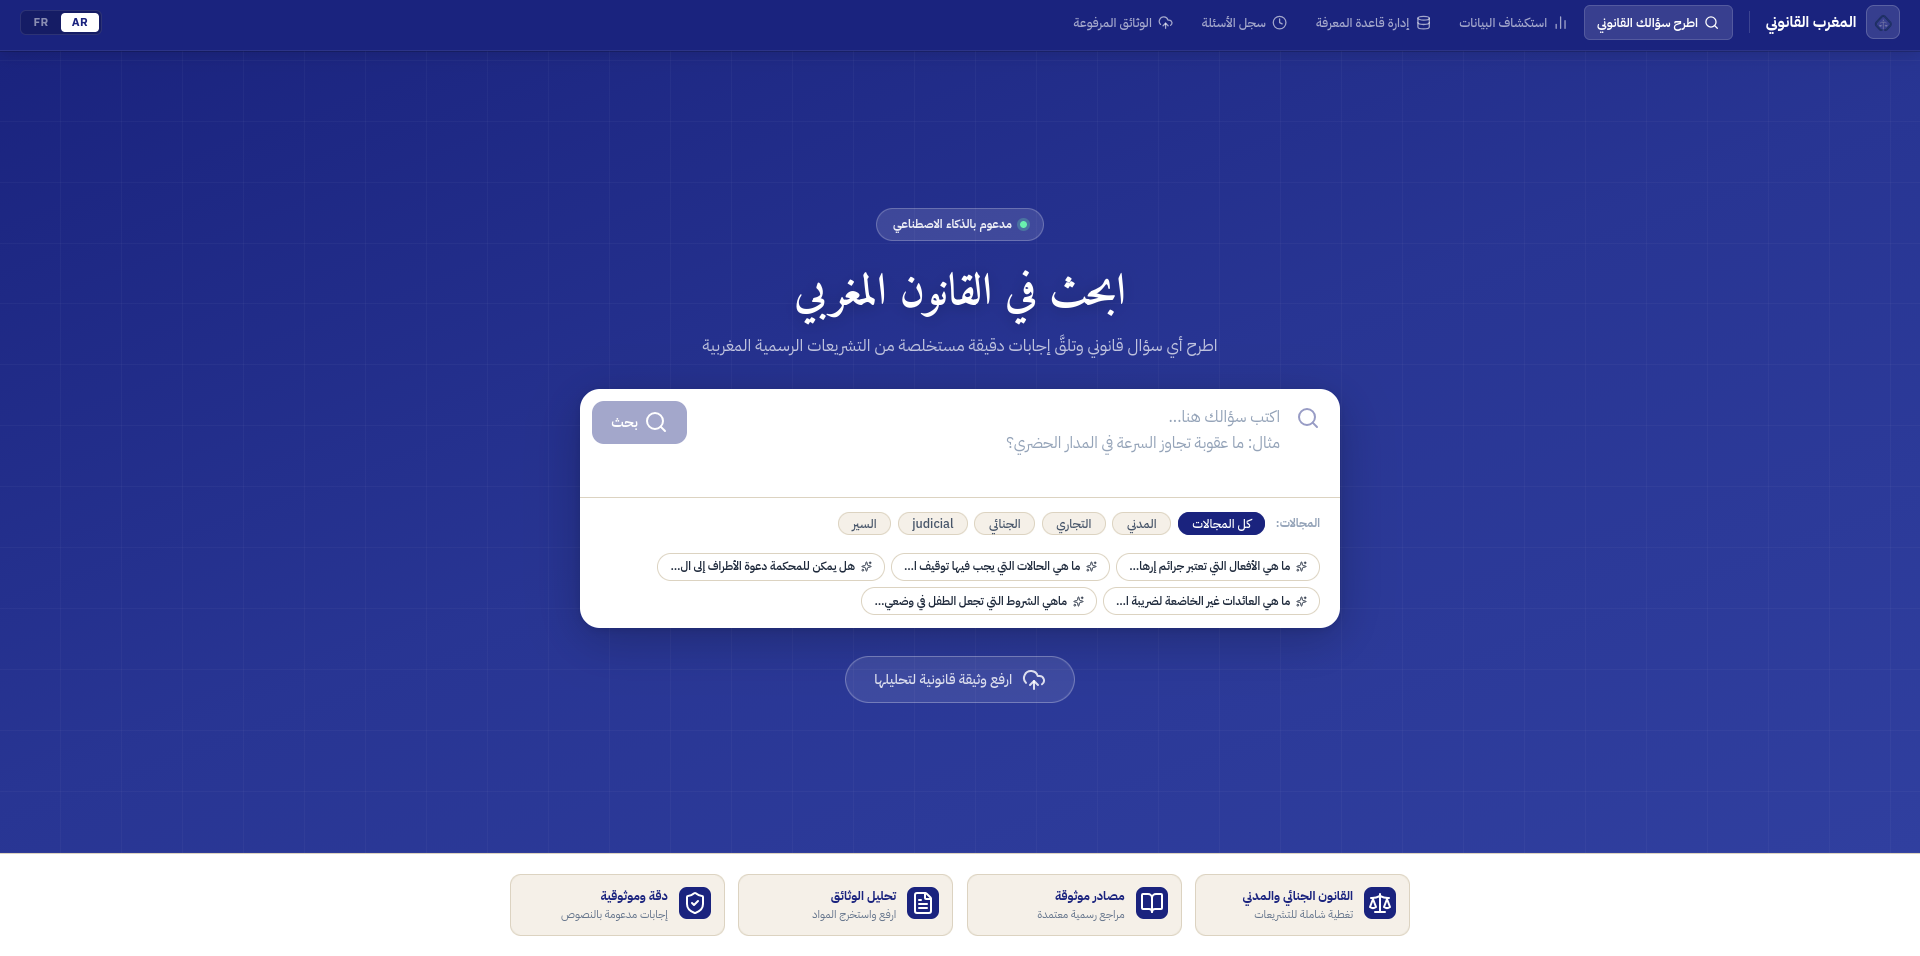
\includegraphics[width=\textwidth]{images/screenshots/home-page.png}
\caption{Homepage of the Moroccan Legal RAG platform.}
\label{fig:home-page}
\end{figure}


\subsection{Exploration de la Base de Connaissances}

Cette interface permet d'explorer directement la base de connaissances juridique indexée par le système. L'utilisateur peut soumettre une requête, sélectionner un domaine juridique et choisir une stratégie de recherche (Dense, BM25 ou Hybride RRF). Elle facilite l'analyse des résultats récupérés et l'évaluation des différentes méthodes de recherche implémentées dans la plateforme.


\begin{figure}[H]
\centering
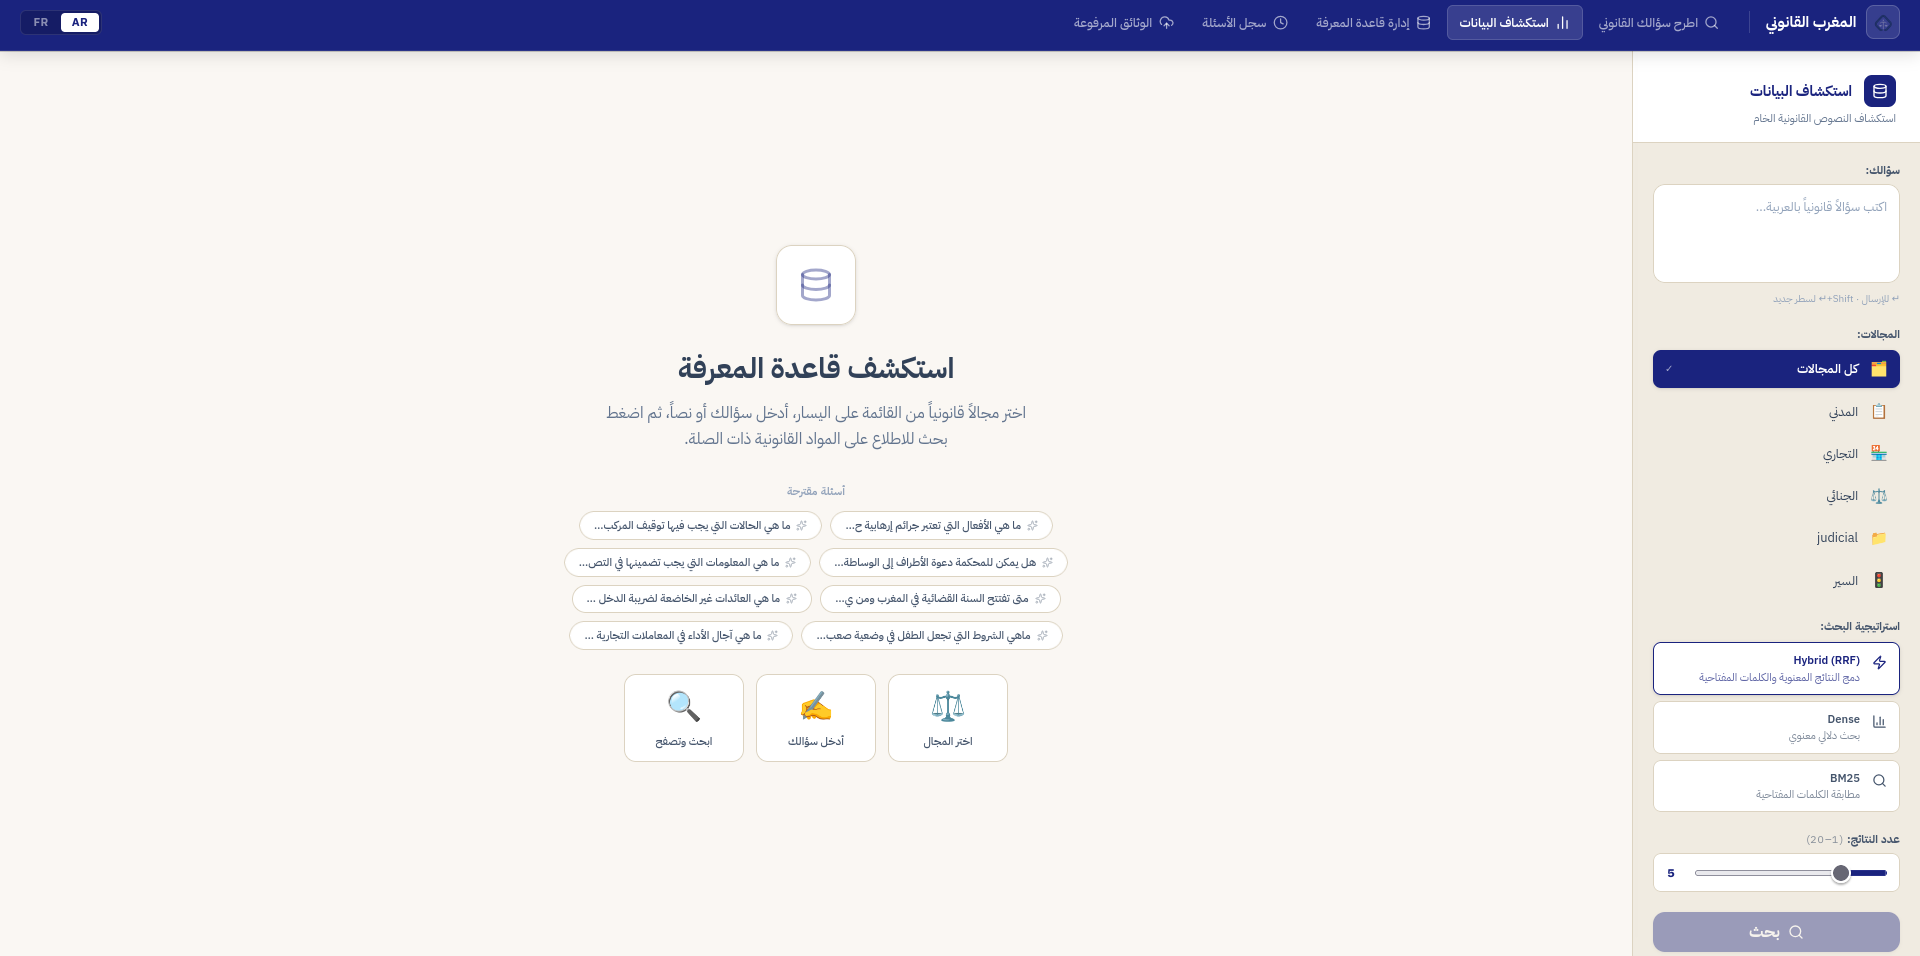
\includegraphics[width=\textwidth]{images/screenshots/knowledge-base-explorer-1.png}
\caption{Interface d'exploration de la base de connaissances juridique.}
\label{fig:knowledge-base-explorer-1}
\end{figure}


\begin{figure}[H]
\centering
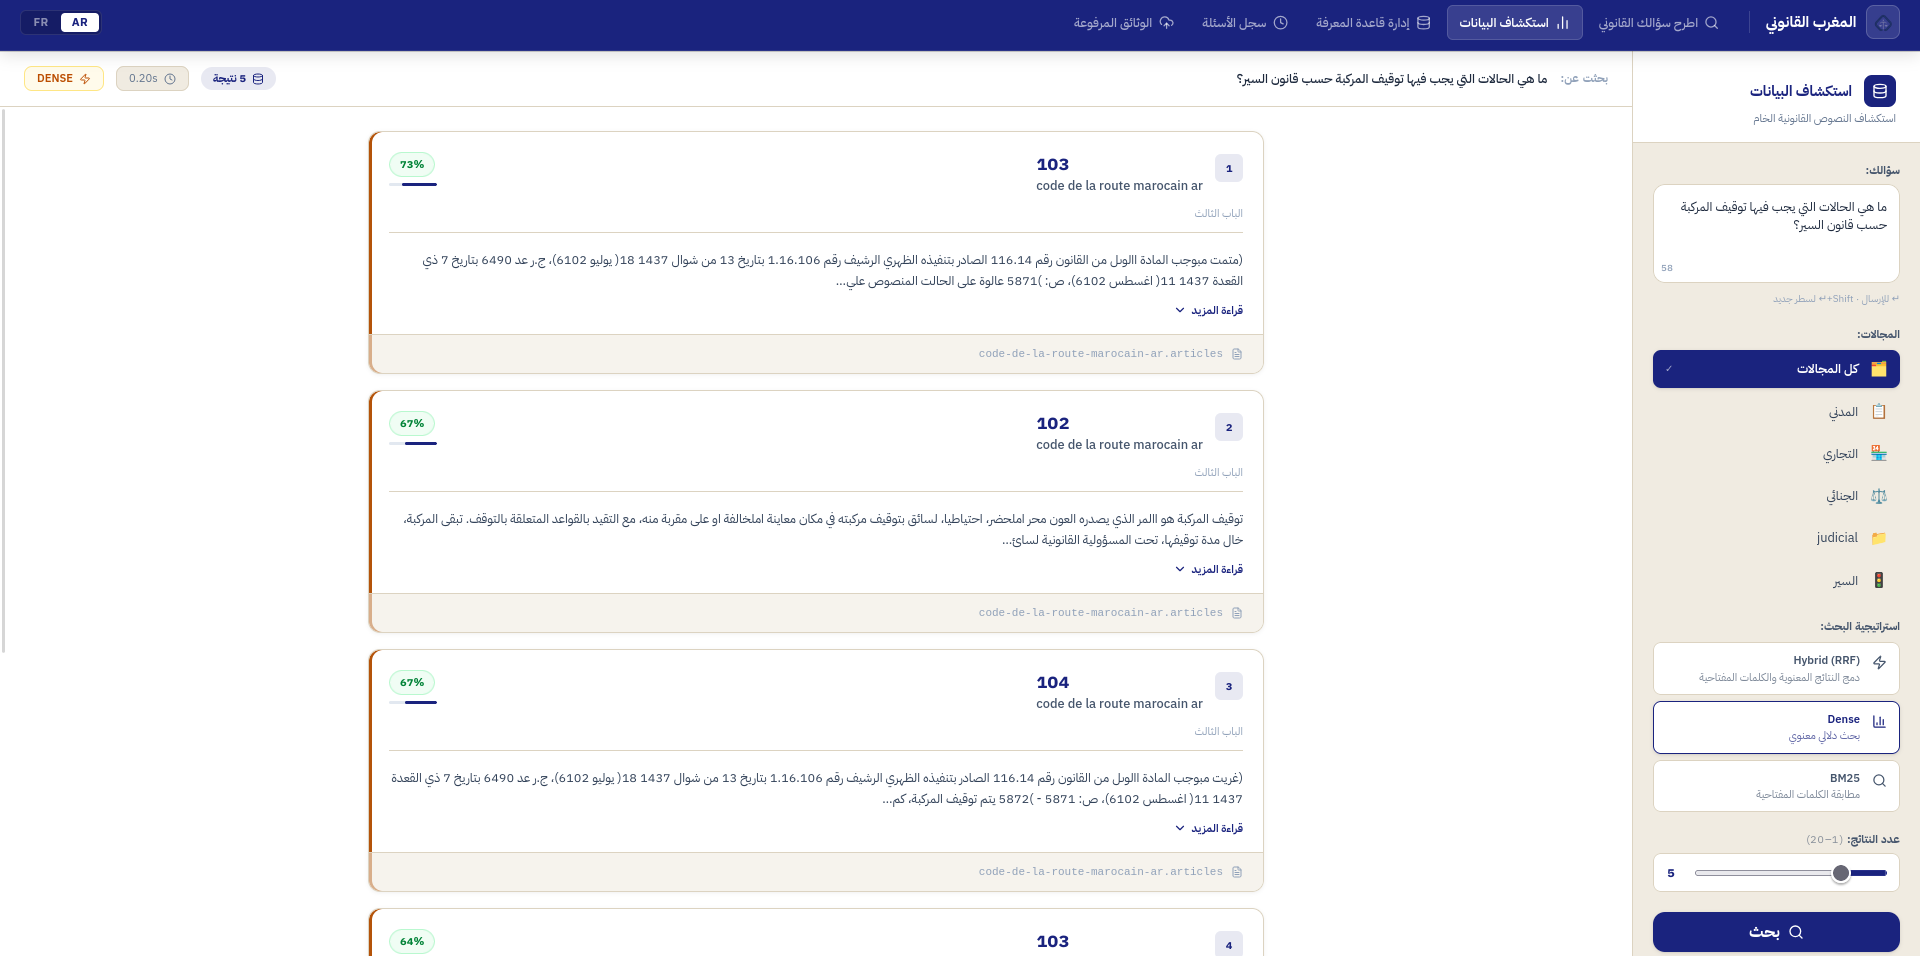
\includegraphics[width=\textwidth]{images/screenshots/knowledge-base-explorer-2.png}
\caption{Interface d'exploration de la base de connaissances juridique.}
\label{fig:knowledge-base-explorer-2}
\end{figure}


\subsection{Gestion de la Base de Connaissances}

Cette interface permet d'administrer les documents juridiques indexés dans la base de connaissances. Elle offre des fonctionnalités de téléversement, de consultation et de gestion des textes législatifs, tout en affichant des statistiques sur le nombre de lois, d'articles et de domaines juridiques disponibles. Les documents peuvent être activés ou désactivés afin de contrôler leur participation au processus de recherche et de génération des réponses.


\begin{figure}[H]
\centering
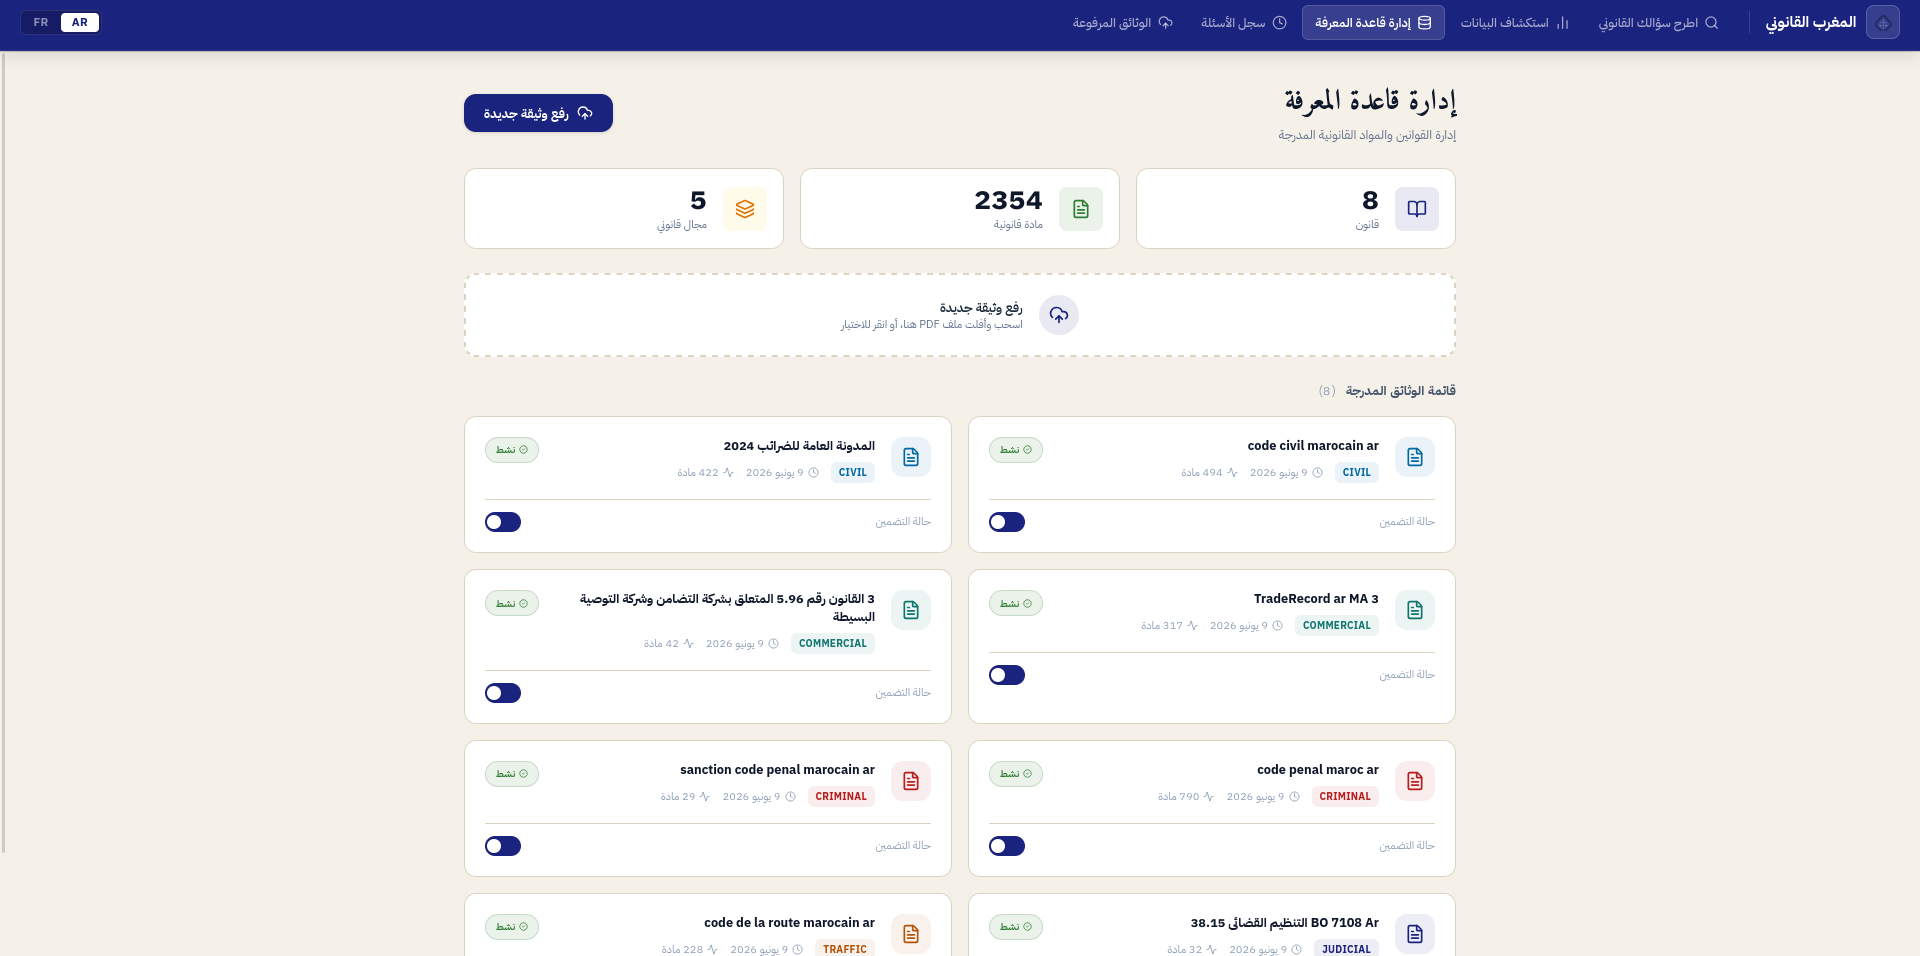
\includegraphics[width=\textwidth]{images/screenshots/knowledge-base-management.png}
\caption{Interface de gestion de la base de connaissances.}
\label{fig:knowledge-base-management}
\end{figure}


\subsection{Historique des Conversations}

Cette interface permet de consulter l'historique des questions posées à la plateforme. Les utilisateurs peuvent rechercher, parcourir et reprendre d'anciennes conversations afin de retrouver rapidement des réponses juridiques précédemment générées. Elle facilite le suivi des échanges et améliore la continuité de l'expérience utilisateur.

\begin{figure}[H]
\centering
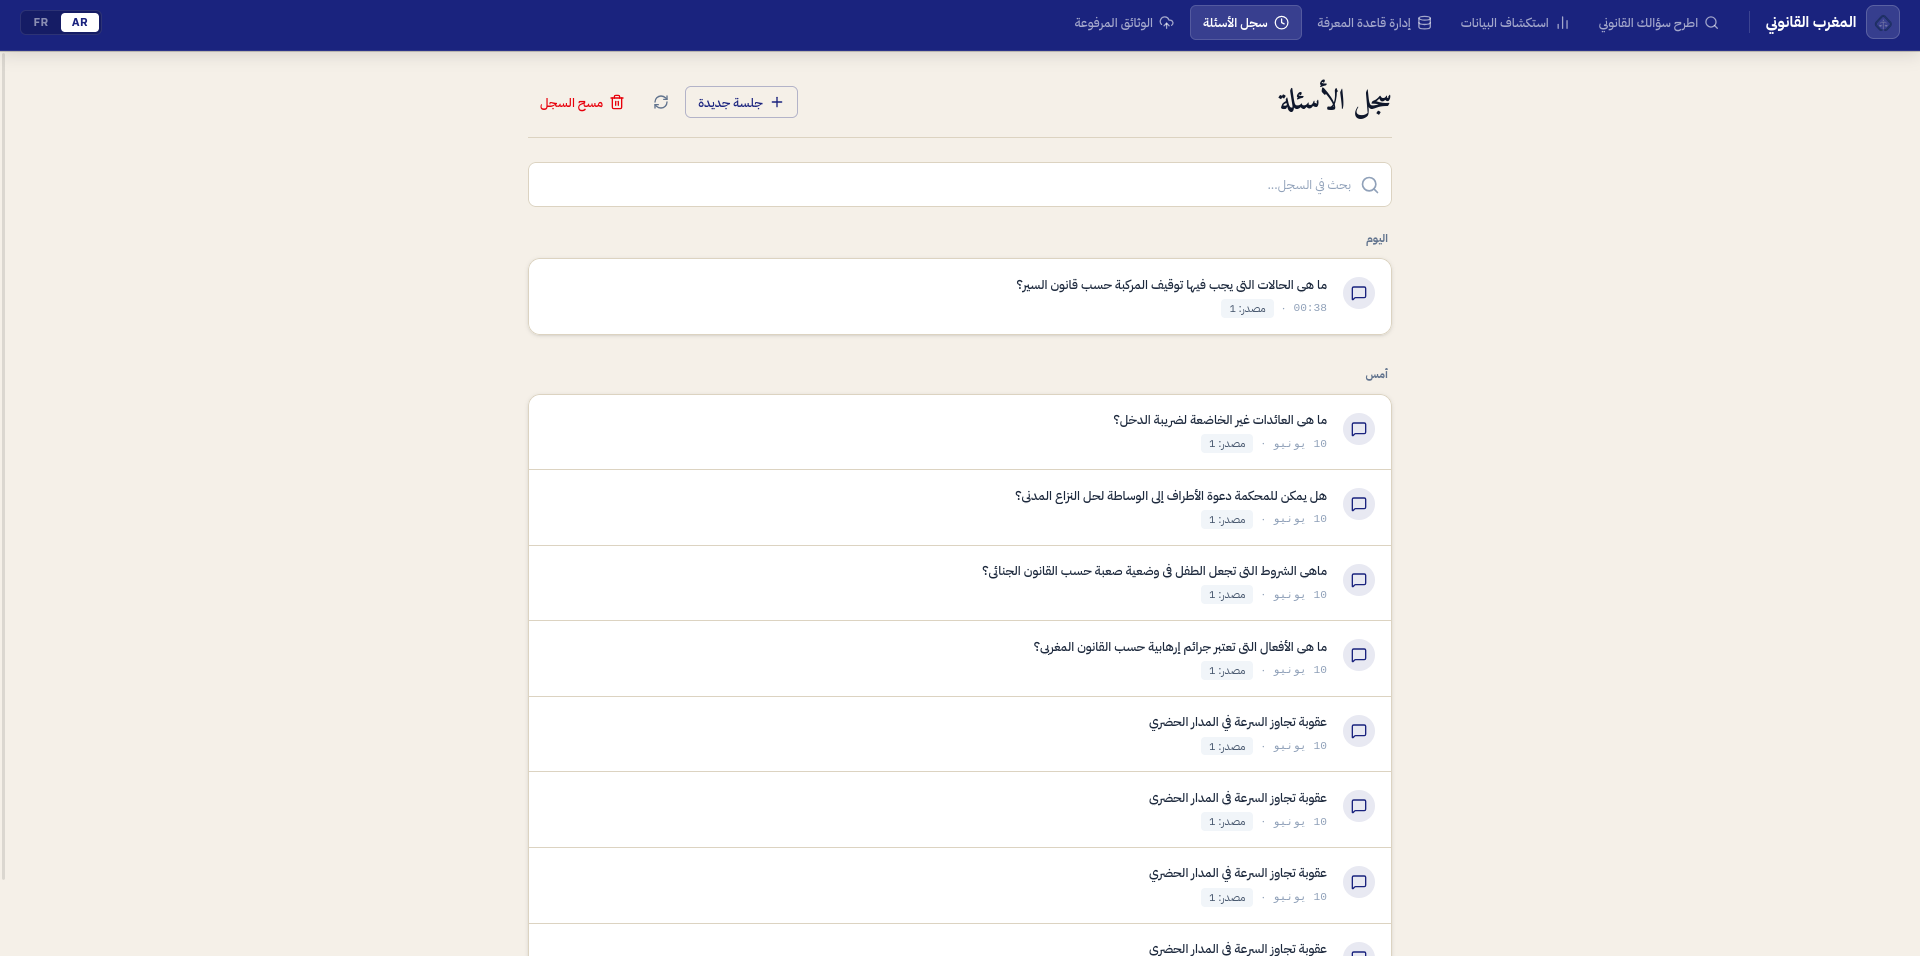
\includegraphics[width=\textwidth]{images/screenshots/conversation-history.png}
\caption{Interface d'historique des conversations.}
\label{fig:conversation-history}
\end{figure}


\subsection{Téléversement et Traitement des Documents Juridiques}

Cette interface permet aux utilisateurs de téléverser des documents juridiques au format PDF pour un traitement automatisé. Le système extrait le contenu du document, identifie les articles juridiques et les transforme en données structurées pouvant être intégrées à la base de connaissances. La page affiche également l'historique des documents traités ainsi que le nombre d'articles extraits pour chaque fichier.


\begin{figure}[H]
\centering
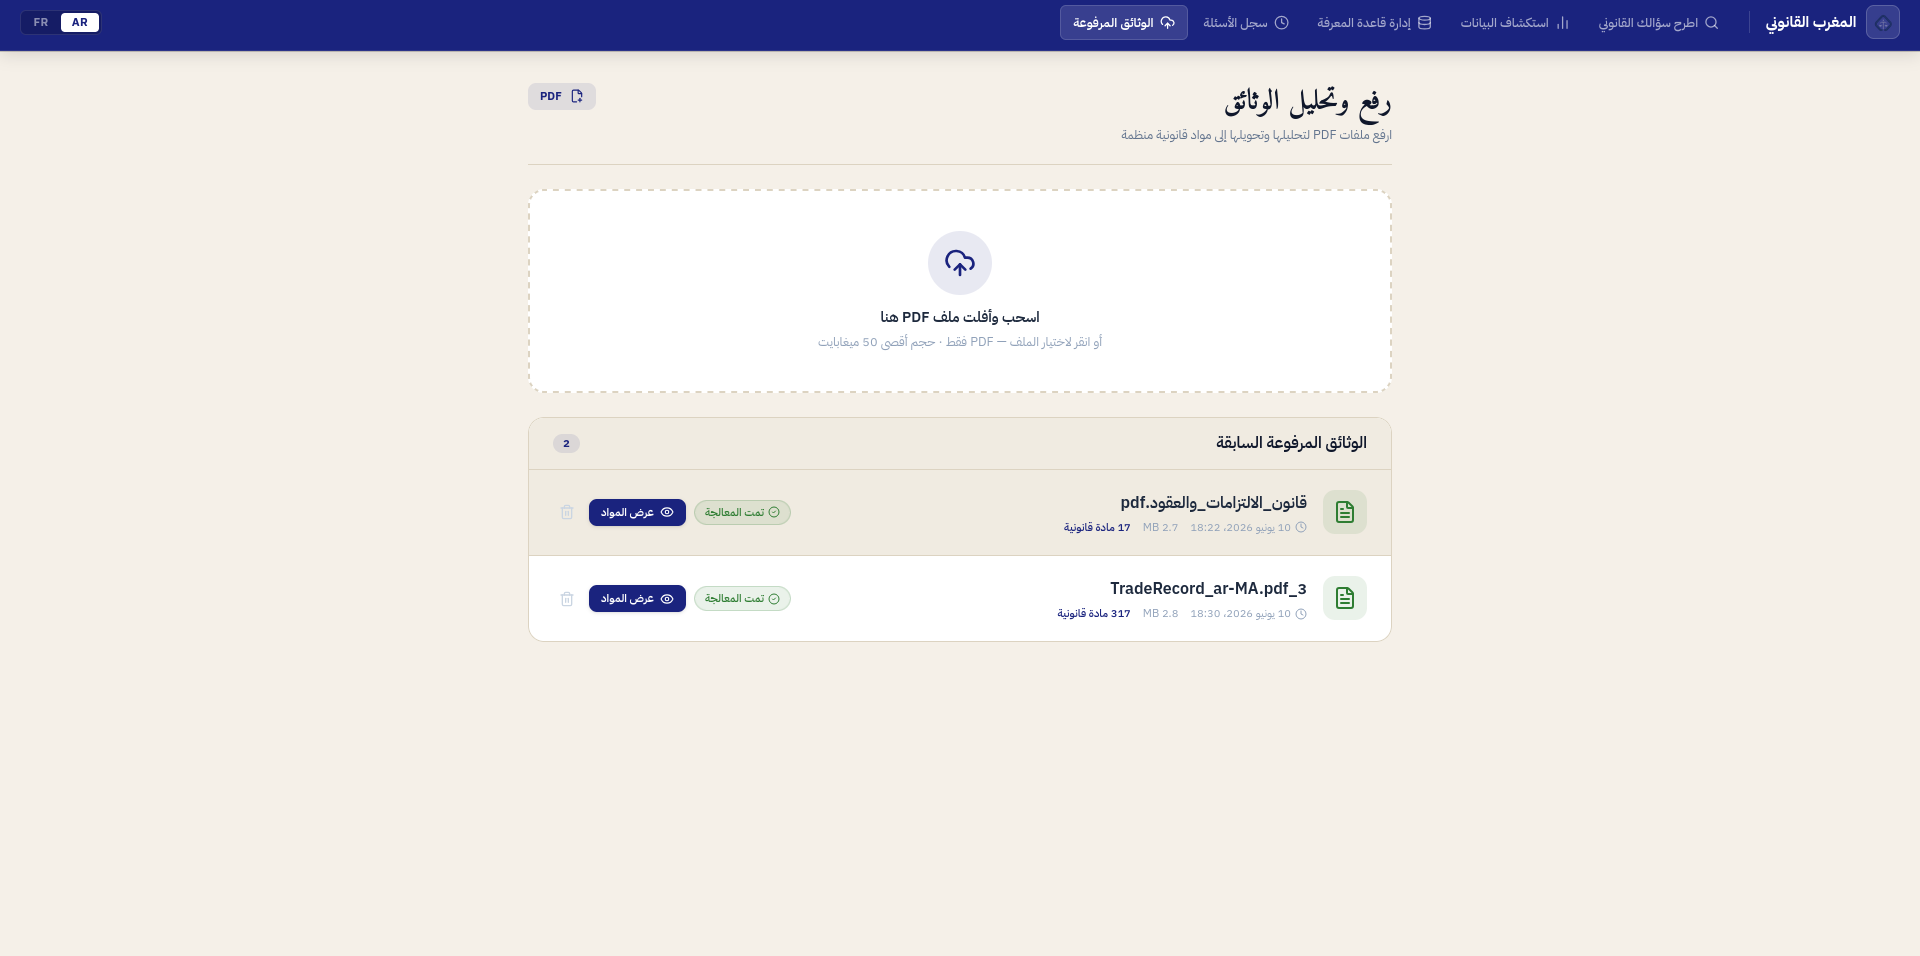
\includegraphics[width=\textwidth]{images/screenshots/document-upload-processing-1.png}
\caption{Interface de téléversement et de traitement des documents juridiques.}
\label{fig:document-upload-processing-1}
\end{figure}

\begin{figure}[H]
\centering
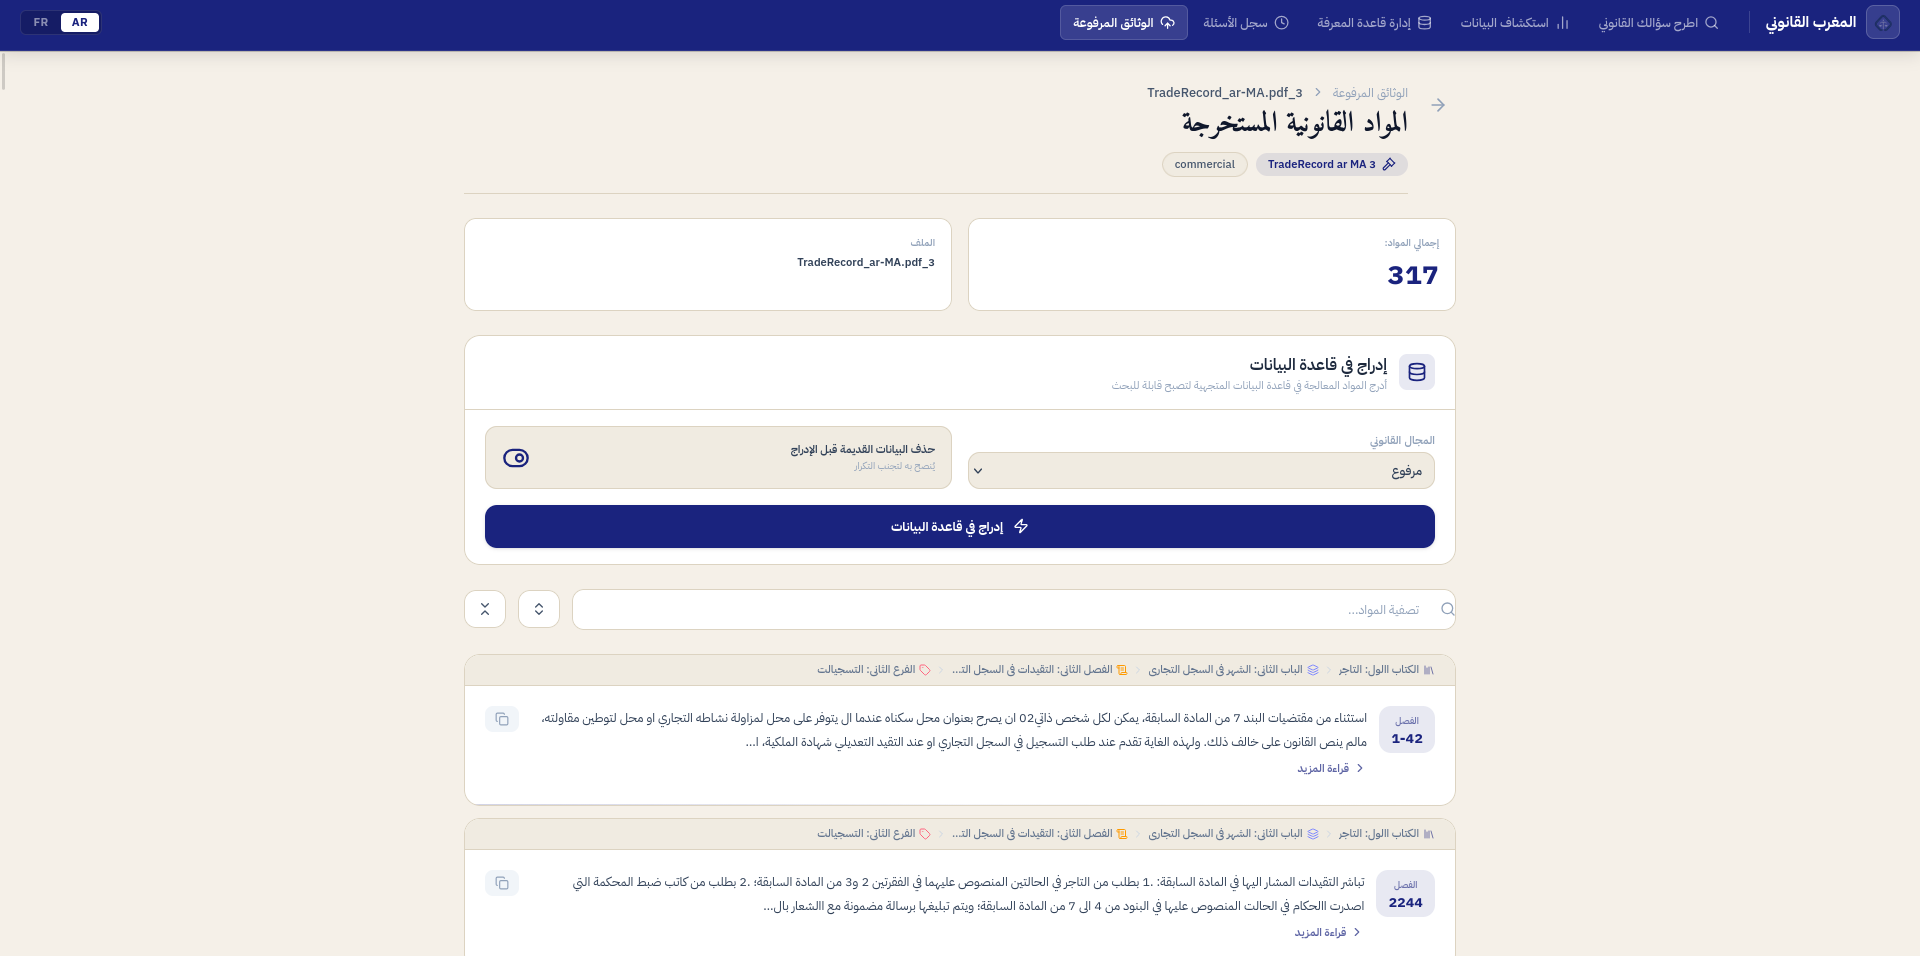
\includegraphics[width=\textwidth]{images/screenshots/document-upload-processing-2.png}
\caption{Interface de téléversement et de traitement des documents juridiques.}
\label{fig:document-upload-processing-2}
\end{figure}


\subsection{Interface Conversationnelle}

Cette interface constitue le cœur du système de question-réponse juridique. Elle affiche la réponse générée par le modèle ainsi que les sources légales utilisées pour sa génération. Les passages juridiques pertinents sont présentés avec leur score de pertinence, permettant à l'utilisateur de vérifier l'origine des informations et d'assurer la transparence du processus de génération.

\begin{figure}[H]
\centering
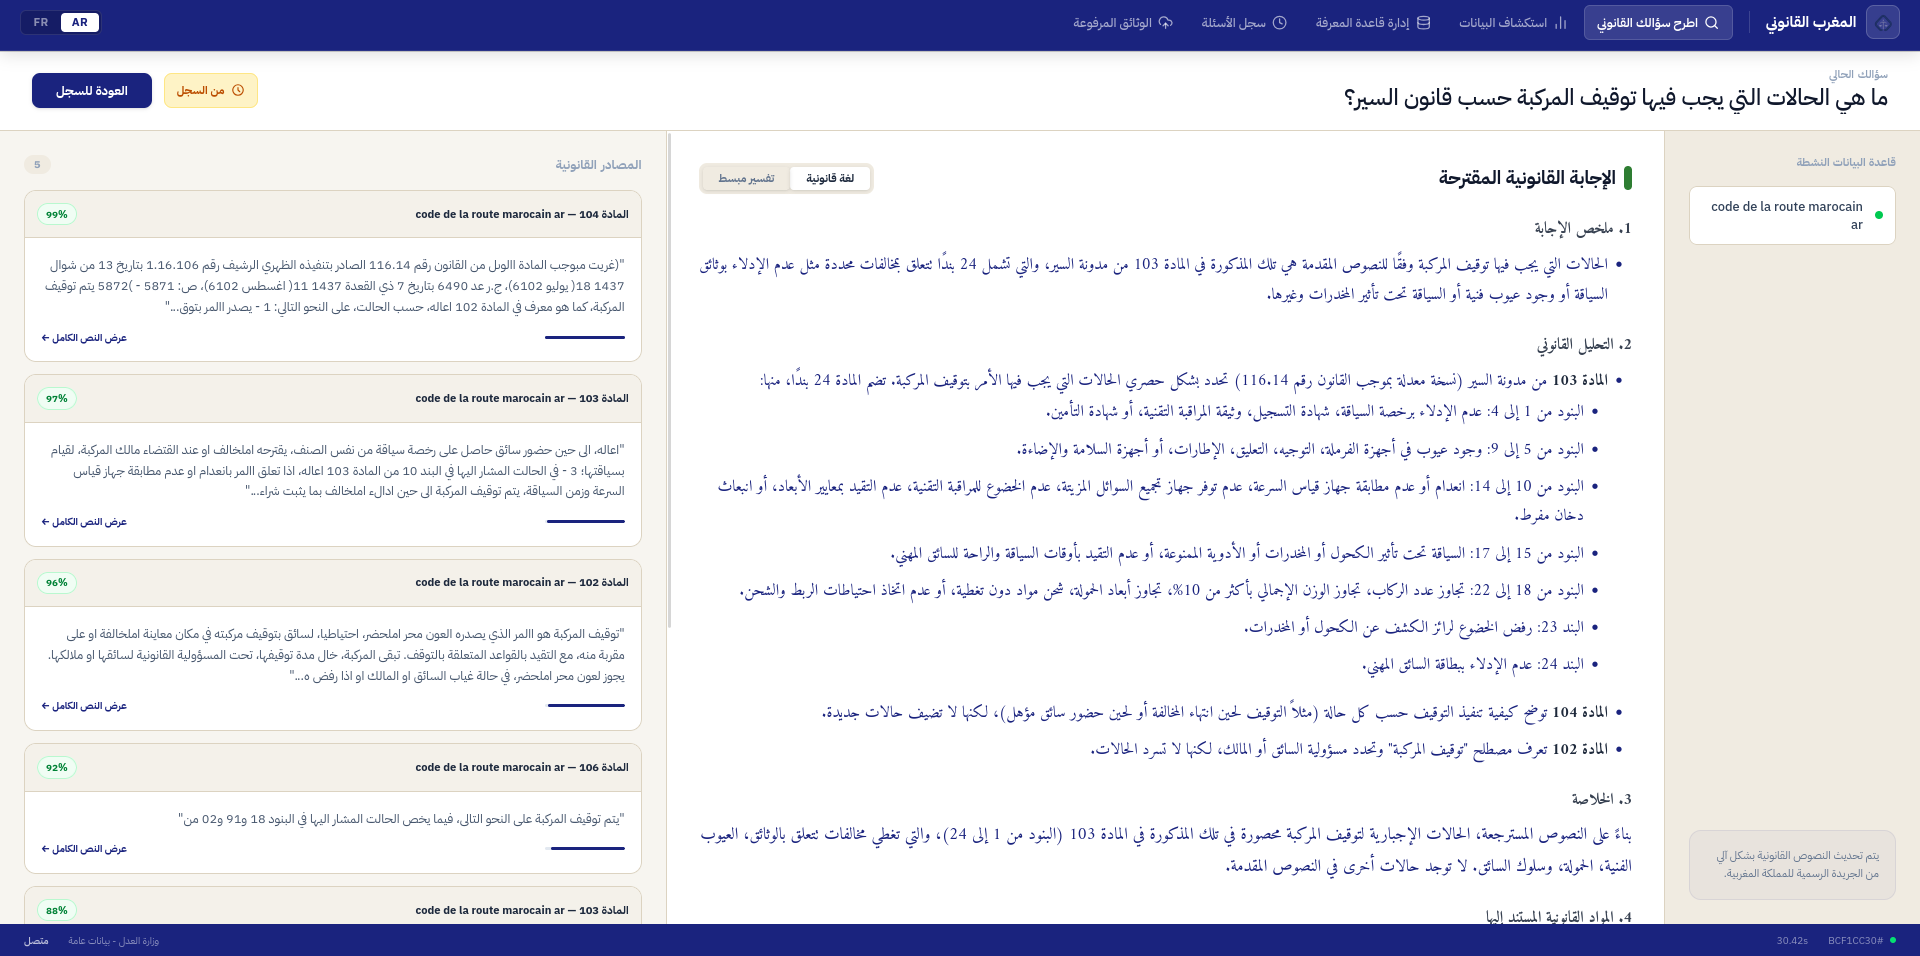
\includegraphics[width=\textwidth]{images/screenshots/conversation-interface.png}
\caption{Interface conversationnelle avec réponses générées et sources juridiques.}
\label{fig:conversation-interface}
\end{figure}
